\documentclass{lmcs}
\usepackage{amssymb,amsmath}
\usepackage{cmll}
\usepackage{txfonts}
\usepackage{graphicx}
\usepackage{stmaryrd}
\usepackage{todonotes}
\usepackage{mathpartir}
\usepackage{hyperref}
\usepackage{mdframed}
\usepackage[barr]{xy}

\newtheorem{theorem}{Theorem}
\newtheorem{lemma}[theorem]{Lemma}
\newtheorem{corollary}[theorem]{Corollary}
\newtheorem{definition}[theorem]{Definition}
\newtheorem{proposition}[theorem]{Proposition}
\newtheorem{example}[theorem]{Example}

%% This renames Barr's \to to \mto.  This allows us to use \to for imp
%% and \mto for a inline morphism.
\let\mto\to
\let\to\relax
\newcommand{\to}{\rightarrow}
\newcommand{\ndto}[1]{\to_{#1}}
\newcommand{\ndwedge}[1]{\wedge_{#1}}

% Commands that are useful for writing about type theory and programming language design.
%% \newcommand{\case}[4]{\text{case}\ #1\ \text{of}\ #2\text{.}#3\text{,}#2\text{.}#4}
\newcommand{\interp}[1]{\llbracket #1 \rrbracket}
\newcommand{\normto}[0]{\rightsquigarrow^{!}}
\newcommand{\join}[0]{\downarrow}
\newcommand{\redto}[0]{\rightsquigarrow}
\newcommand{\nat}[0]{\mathbb{N}}
\newcommand{\fun}[2]{\lambda #1.#2}
\newcommand{\CRI}[0]{\text{CR-Norm}}
\newcommand{\CRII}[0]{\text{CR-Pres}}
\newcommand{\CRIII}[0]{\text{CR-Prog}}
\newcommand{\subexp}[0]{\sqsubseteq}
%% Must include \usepackage{mathrsfs} for this to work.

\date{}

\let\b\relax
\let\d\relax
\let\t\relax
\let\r\relax
\let\c\relax
\let\j\relax
\let\wn\relax
\let\H\relax

% Cat commands.
\newcommand{\powerset}[1]{\mathcal{P}(#1)}
\newcommand{\cat}[1]{\mathcal{#1}}
\newcommand{\func}[1]{\mathsf{#1}}
\newcommand{\iso}[0]{\mathsf{iso}}
\newcommand{\H}[0]{\func{H}}
\newcommand{\J}[0]{\func{J}}
\newcommand{\catop}[1]{\cat{#1}^{\mathsf{op}}}
\newcommand{\Hom}[3]{\mathsf{Hom}_{\cat{#1}}(#2,#3)}
\newcommand{\limp}[0]{\multimap}
\newcommand{\colimp}[0]{\multimapdotinv}
\newcommand{\dial}[1]{\mathsf{Dial_{#1}}(\mathsf{Sets^{op}})}
\newcommand{\dialSets}[1]{\mathsf{Dial_{#1}}(\mathsf{Sets})}
\newcommand{\dcSets}[1]{\mathsf{DC_{#1}}(\mathsf{Sets})}
\newcommand{\sets}[0]{\mathsf{Sets}}
\newcommand{\obj}[1]{\mathsf{Obj}(#1)}
\newcommand{\mor}[1]{\mathsf{Mor(#1)}}
\newcommand{\id}[0]{\mathsf{id}}
\newcommand{\lett}[0]{\mathsf{let}\,}
\newcommand{\inn}[0]{\,\mathsf{in}\,}
\newcommand{\cur}[1]{\mathsf{cur}(#1)}
\newcommand{\curi}[1]{\mathsf{cur}^{-1}(#1)}
\newcommand{\m}[1]{\mathsf{m}_{#1}}
\newcommand{\n}[1]{\mathsf{n}_{#1}}
\newcommand{\b}[1]{\mathsf{b}_{#1}}
\newcommand{\d}[1]{\mathsf{d}_{#1}}
\newcommand{\h}[1]{\mathsf{h}_{#1}}
\newcommand{\p}[1]{\mathsf{p}_{#1}}
\newcommand{\q}[1]{\mathsf{q}_{#1}}
\newcommand{\t}[0]{\mathsf{t}}
\newcommand{\r}[1]{\mathsf{r}_{#1}}
\newcommand{\s}[1]{\mathsf{s}_{#1}}
\newcommand{\w}[1]{\mathsf{w}_{#1}}
\newcommand{\c}[1]{\mathsf{c}_{#1}}
\newcommand{\j}[1]{\mathsf{j}_{#1}}
\newcommand{\jinv}[1]{\mathsf{j}^{-1}_{#1}}
\newcommand{\wn}[0]{\mathop{?}}
\newcommand{\codiag}[1]{\bigtriangledown_{#1}}

\newenvironment{changemargin}[2]{%
  \begin{list}{}{%
    \setlength{\topsep}{0pt}%
    \setlength{\leftmargin}{#1}%
    \setlength{\rightmargin}{#2}%
    \setlength{\listparindent}{\parindent}%
    \setlength{\itemindent}{\parindent}%
    \setlength{\parsep}{\parskip}%
  }%
  \item[]}{\end{list}}

\newenvironment{diagram}{
  \begin{center}
    \begin{math}
      \bfig
}{
      \efig
    \end{math}
  \end{center}
}

%% Ott
\input{DualLNL-inc}

\urldef{\mailsa}\path|{heades}@augusta.edu|

\begin{document}

\title{A Cointuitionistic Adjoint Logic}
\author{Harley Eades III}
\email{heades@augusta.edu}
\address{Computer Science, Augusta University, Augusta, GA}

\author{Gianluigi Bellin}
\email{gianluigi.bellin@univr.it}
\address{Dipartimento di Informatica, Universit\`{a} di Verona, Strada Le Grazie, 37134 Verona, Italy}

\maketitle 

\begin{abstract}

  

\end{abstract}

\section{Introduction}
\label{sec:introduction}
Bi-intuitionistic logic (BINT) is a conservative extension of
intuitionistic logic with perfect duality.  That is, BINT contains the
usual intuitionistic logical connectives such as true, conjunction,
and implication, but also their duals false, disjunction, and
coimplication. One leading question with respect to BINT is, what does
BINT look like across the three arcs -- logic, typed
$\lambda$-calculi, and category theory -- of the Curry-Howard-Lambek
correspondence?  A non-trivial (does not degenerate to a poset)
categorical model of BINT is currently an open problem.  This paper is
the first of two that will provide an answer to this open problem.

BINT can be seen as a mixing of two worlds: the first being
intuitionistic logic (IL), which is modeled categorically by a
cartesian closed category (CCC), and the second being the dual to
intuitionistic logic called cointuitionistic logic (coIL), which is
modeled by a cocartesian coclosed category (coCCC).  Crolard
\cite{Crolard:2001} showed that combining these two categories into
the same category results in it degenerating to a poset, that is,
there is at most one morphism between any two objects; we review this
result in
Section~\ref{subsec:cartesian_closed_and_cocartesian_coclosed_categories}.
However, this degeneration does not occur when both logics are linear.
We propose that these two worlds need to be separated, and then mixed
in a control way using the modalities from linear logic.  This
separation can be ultimately achieved by an adjoint formalization of
bi-intuitionistic logic.  This formalization consists of three worlds
instead of two: the first is intuitionistic logic, the second is
linear bi-intuitionistic (Bi-ILL), and the third is cointuitionistic
logic.  They are then related via two adjunctions as depicted by the
following diagram:
\begin{center}
  \begin{tikzpicture}
    \node (img) {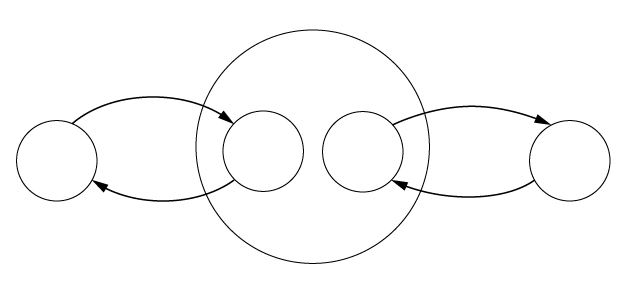
\includegraphics[scale=0.4]{introDiag}};
    \node (dv) at (-2.3, 0.0) {\huge $\dashv$};
    \node (IL) at (-3.58, -0.1) {IL};
    \node (vd) at (2.3, 0.0) {\huge $\vdash$};
    \node (coIL) at (3.65, -0.1) {coIL};

    \node (ILL) at (-0.67, 0.0) {ILL};
    \node (coILL) at (0.71, 0.0) {coILL};
    \node (BiILL) at (0, 1.0) {Bi-ILL};
  \end{tikzpicture}
    
\end{center}
The adjoint between IL and ILL is known as a LNL model of ILL, and is
due to Benton \cite{Benton:1994}.  However, the dual to LNL models
which would amount to the adjoint between coILL and coIL has yet to
appear in the literature.

The main contribution of this paper is the definition and study of the
dual to Benton's LNL models as models of cointuitionistic logic called
dual LNL models.  Bellin \cite{Bellin:2012} was the first to propose
the dual to Bierman's \cite{Bierman:1994} linear categories which he
names dual linear categories as a model of cointuitionistic linear
logic.  We conduct a similar analysis to that of Benton for dual LNL
models by showing that dual LNL models are dual linear categories
(Section~\ref{subsec:dual_lnl_model_implies_dual_category}), and that
from a dual linear category we may obtain a dual LNL model
(Section~\ref{subsec:dual_category_implies_dual_lnl_model}).
Following this we give the definition of bi-LNL models by combining
our dual LNL models with Benton's LNL models to obtain a categorical
model of bi-intuitionistic logic
(Section~\ref{subsec:a_mixed_bi-linear_non-linear_model}), but we
leave its analysis and corresponding logic to a future paper.
Finally, we give the definition of dual LNL logic with a term
assignment (Section~\ref{sec:dual_lnl_logic} and
Section~\ref{sec:dual_lnl_term_assignment} respectively).
% section introduction (end)

\section{The Adjoint Model}
\label{sec:adjoint_model}

Suppose $(\cat{I}, 1, \times, \to)$ is a cartesian closed category,
and $(\cat{L}, \top, \otimes, \limp)$ is a symmetric monoidal closed
category.  Then relate these two categories with a symmetric monoidal
adjunction $\cat{I} : \func{F} \dashv \func{G} : \cat{L}$
(Definition~\ref{def:SMCADJ}), where $\func{F}$ and $\func{G}$ are
symmetric monoidal functors.  The later point implies that there are
natural transformations $\m{X,Y} : \func{F}X \otimes \func{F}Y \mto
\func{F}(X \times Y)$ and $\n{A,B} : \func{G}A \times \func{G}B \mto
\func{G}(A \otimes B)$, and maps $\m\top : \top \mto \func{F}1$ and
$\n1 : 1 \mto \func{G}\top$ subject to several coherence conditions;
see Definition~\ref{def:SMCFUN}.  Furthermore, the functor $\func{F}$
is strong which means that $\m{X,Y}$ and $\m{\top}$ are isomorphisms.
This setup turns out to be one of the most beautiful models of
intuitionistic linear logic called a LNL model due to Benton
\cite{Benton:1994}.  In fact, the linear modality of-course can be
defined by $!A = \func{F}(\func{G}(A))$ which defines a symmetric
monoidal comonad using the adjunction; see Section~2.2 of
\cite{Benton:1994}.  This model is much simpler than other known
models, and resulted in a logic called LNL logic which supports mixing
intuitionistic logic with linear logic.  This type of model leads to
an elegant and useful model of bi-intuitionism.

Taking the dual of the previous model results in what we call dual LNL
models. They consist of a cocartesian coclosed category, $(\cat{C}, 0,
+, -)$, a symmetric monoidal coclosed category, $(\cat{L}', \perp,
\oplus, \colimp)$, where $\colimp : \cat{L}' \times \cat{L}' \mto
\cat{L}'$ is left adjoint to cotensor (sometimes called parr), and a
symmetric comonoidal adjunction (Definition~\ref{def:coSMCADJ})
$\cat{L'} : \func{H} \dashv \func{J} : \cat{C}$.  We will show that dual LNL
models are a simplification of dual linear categories as defined by
Bellin \cite{Bellin:2012} in much of the same way that LNL models are
a simplification of linear categories.  In fact, we will define
Girard's exponential why-not by $\wn A = \func{JH}A$, and hence, is the
monad induced by the adjunction.

\subsection{Symmetric (co)Monoidal Categories}
\label{subsec:symmetric_monoidal_categories}
We now introduce the necessary definitions related to symmetric
monoidal categories that our model will depend on.  Most of these
definitions are equivalent to the ones given by Benton
\cite{Benton:1994}, but we give a lesser known definition of symmetric
comonoidal functors due to Bellin \cite{Bellin:2012}.  In this
section we also introduce distributive categories, the notion of
cocloser, and finally, the definition of bilinear categories.  The
reader may wish to simply skim this section, but refer back to it when
they encounter a definition or result they do not know.

\begin{definition}
  \label{def:monoidal-category}
  A \textbf{symmetric monoidal category (SMC)} is a category, $\cat{M}$,
  with the following data:
  \begin{itemize}
  \item An object $\top$ of $\cat{M}$,
  \item A bi-functor $\otimes : \cat{M} \times \cat{M} \mto \cat{M}$,
  \item The following natural isomorphisms:
    \[
    \begin{array}{lll}
      \lambda_A : \top \otimes A \mto A\\
      \rho_A : A \otimes \top \mto A\\      
      \alpha_{A,B,C} : (A \otimes B) \otimes C \mto A \otimes (B \otimes C)\\
    \end{array}
    \]
  \item A symmetry natural transformation:
    \[
    \beta_{A,B} : A \otimes B \mto B \otimes A
    \]
  \item Subject to the following coherence diagrams:
    \begin{mathpar}
      \bfig
      \vSquares|ammmmma|/->`->```->``<-/[
        ((A \otimes B) \otimes C) \otimes D`
        (A \otimes (B \otimes C)) \otimes D`
        (A \otimes B) \otimes (C \otimes D)``
        A \otimes (B \otimes (C \otimes D))`
        A \otimes ((B \otimes C) \otimes D);
        \alpha_{A,B,C} \otimes \id_D`
        \alpha_{A \otimes B,C,D}```
        \alpha_{A,B,C \otimes D}``
        \id_A \otimes \alpha_{B,C,D}]      
      
      \morphism(1206,1000)|m|<0,-1000>[
        (A \otimes (B \otimes C)) \otimes D`
        A \otimes ((B \otimes C) \otimes D);
        \alpha_{A,B \otimes C,D}]
      \efig
      \and
      \bfig
      \hSquares|aammmaa|/->`->`->``->`->`->/[
        (A \otimes B) \otimes C`
        A \otimes (B \otimes C)`
        (B \otimes C) \otimes A`
        (B \otimes A) \otimes C`
        B \otimes (A \otimes C)`
        B \otimes (C \otimes A);
        \alpha_{A,B,C}`
        \beta_{A,B \otimes C}`
        \beta_{A,B} \otimes \id_C``
        \alpha_{B,C,A}`
        \alpha_{B,A,C}`
        \id_B \otimes \beta_{A,C}]
      \efig      
    \end{mathpar}
    \begin{mathpar}
      \bfig
      \Vtriangle[
        (A \otimes \top) \otimes B`
        A \otimes (\top \otimes B)`
        A \otimes B;
        \alpha_{A,\top,B}`
        \rho_{A}`
        \lambda_{B}]
      \efig
      \and
      \bfig
      \btriangle[
        A \otimes B`
        B \otimes A`
        A \otimes B;
        \beta_{A,B}`
        \id_{A \otimes B}`
        \beta_{B,A}]
      \efig
      \and
      \bfig
      \Vtriangle[
        \top \otimes A`
        A \otimes \top`
        A;
        \beta_{\top,A}`
        \lambda_A`
        \rho_A]
      \efig
    \end{mathpar}    
  \end{itemize}
\end{definition}

Categorical modeling implication requires that the model be closed;
which can be seen as an internalization of the notion of a morphism.
\begin{definition}
  \label{def:SMCC}
  A \textbf{symmetric monoidal closed category (SMCC)} is a symmetric
  monoidal category, $(\cat{M},\top,\otimes)$, such that, for any object
  $B$ of $\cat{M}$, the functor $- \otimes B : \cat{M} \mto \cat{M}$
  has a specified right adjoint.  Hence, for any objects $A$ and $C$
  of $\cat{M}$ there is an object $B \limp C$ of $\cat{M}$ and a
  natural bijection:
  \[
  \Hom{\cat{M}}{A \otimes B}{C} \cong \Hom{\cat{M}}{A}{B \limp C}
  \]
  We call the functor $\limp : \cat{M} \times \cat{M} \mto \cat{M}$
  the internal hom of $\cat{M}$.
\end{definition}

Symmetric monoidal closed categories can be seen as a model of
intuitionistic linear logic with a tensor product and implication.
What happens when we take the dual?  First, we have the following
result:
\begin{lemma}[Dual of Symmetric Monoidal Categories]
  \label{lemma:dual_of_symmetric_monoidal_categories}
  If $(\cat{M},\top,\otimes)$ is a symmetric monoidal category, then
  $\catop{M}$ is also a symmetric monoidal category.
\end{lemma}
The previous result follows from the fact that the structures making
up symmetric monoidal categories are isomorphisms, and so naturally
taking their opposite will yield another symmetric monoidal category.
To emphasize when we are thinking about a symmetric monoidal category
in the opposite we use the notation $(\cat{M},\perp,\oplus)$ which gives
the suggestion of $\oplus$ corresponding to a disjunctive tensor
product which we call the \textit{cotensor} of $\cat{M}$. The next
definition describes when a symmetric monoidal category is coclosed.
\begin{definition}
  \label{def:SMCC}
  A \textbf{symmetric monoidal coclosed category (SMCCC)} is a symmetric
  monoidal category, $(\cat{M},\perp,\oplus)$, such that, for any object
  $B$ of $\cat{M}$, the functor $- \oplus B : \cat{M} \mto \cat{M}$
  has a specified left adjoint.  Hence, for any objects $A$ and $C$
  of $\cat{M}$ there is an object $C \colimp B$ of $\cat{M}$ and a
  natural bijection:
  \[
  \Hom{\cat{M}}{C}{A \oplus B} \cong \Hom{\cat{M}}{C \colimp B}{A}
  \]
  We call the functor $\colimp : \cat{M} \times \cat{M} \mto \cat{M}$
  the internal cohom of $\cat{M}$.
\end{definition}

We combine a symmetric monoidal closed category with a symmetric
monoidal coclosed category in a single category.  First, we define the
notion of a distributive category due to Cockett and Seely
\cite{Cockett:1997}.
\begin{definition}
  \label{def:dist-cat}
  We call a symmetric monoidal category, $(\cat{M}, \top, \otimes,
  \perp, \oplus)$ equipped with the structure of a cotensor $(\cat{M},
  \perp, \oplus)$, a \textbf{distributive category} if there are
  natural transformations:
  \[
  \begin{array}{lll}
    \delta^L_{A,B,C} : A \otimes (B \oplus C) \mto (A \otimes B) \oplus C\\
    \delta^R_{A,B,C} : (B \oplus C) \otimes A \mto B \oplus (C \otimes A)
  \end{array}
  \]
  subject to several coherence diagrams.  Due to the large number of
  coherence diagrams we do not list them here, but they all can be
  found in Cockett and Seely's paper \cite{Cockett:1997}.
\end{definition}
\noindent
Requiring that the tensor and cotensor products have the corresponding
right and left adjoints results in the following definition.
\begin{definition}
  \label{def:bilinear-cat}
  A \textbf{bilinear category} is a distributive category $(\cat{M},
  \top, \otimes, \perp, \oplus)$ such that $(\cat{M}, \top, \otimes)$
  is closed, and $(\cat{M}, \perp, \oplus)$ is coclosed.  We will
  denote bi-linear categories by $(\cat{M}, \top, \otimes, \limp, \perp,
  \oplus, \colimp)$.
\end{definition}
Originally, Lambek defined bilinear categories to be similar to the
previous definition, but the tensor and cotensor were non-commutative
\cite{Cockett:1997a}, however, the bilinear categories given here
are. We retain the name in homage to his original work.  As we will
see below bilinear categories form the core of a categorical model for
bi-intuitionism.

A symmetric monoidal category is a category with additional structure
subject to several coherence diagrams.  Thus, an ordinary functor is
not enough to capture this structure, and hence, the introduction of
symmetric monoidal functors.
\begin{definition}
  \label{def:SMCFUN}
  Suppose we are given two symmetric monoidal
  categories\\ $(\cat{M}_1,\top_1,\otimes_1,\alpha_1,\lambda_1,\rho_1,\beta_1)$
  and
  $(\cat{M}_2,\top_2,\otimes_2,\alpha_2,\lambda_2,\rho_2,\beta_2)$.
  Then a \textbf{symmetric monoidal functor} is a functor $F :
  \cat{M}_1 \mto \cat{M}_2$, a map $m_{\top_1} : \top_2 \mto F\top_1$
  and a natural transformation $m_{A,B} : FA \otimes_2 FB \mto F(A
  \otimes_1 B)$ subject to the following coherence conditions:
  \begin{mathpar}
    \bfig
    \vSquares|ammmmma|/->`->`->``->`->`->/[
      (FA \otimes_2 FB) \otimes_2 FC`
      FA \otimes_2 (FB \otimes_2 FC)`
      F(A \otimes_1 B) \otimes_2 FC`
      FA \otimes_2 F(B \otimes_1 C)`
      F((A \otimes_1 B) \otimes_1 C)`
      F(A \otimes_1 (B \otimes_1 C));
      {\alpha_2}_{FA,FB,FC}`
      m_{A,B} \otimes \id_{FC}`
      \id_{FA} \otimes m_{B,C}``
      m_{A \otimes_1 B,C}`
      m_{A,B \otimes_1 C}`
      F{\alpha_1}_{A,B,C}]
    \efig
    \end{mathpar}
%    \and
\begin{mathpar}
    \bfig
    \square|amma|/->`->`<-`->/<1000,500>[
      \top_2 \otimes_2 FA`
      FA`
      F\top_1 \otimes_2 FA`
      F(\top_1 \otimes_1 A);
      {\lambda_2}_{FA}`
      m_{\top_1} \otimes \id_{FA}`
      F{\lambda_1}_{A}`
      m_{\top_1,A}]
    \efig
    \and
    \bfig
    \square|amma|/->`->`<-`->/<1000,500>[
      FA \otimes_2 \top_2`
      FA`
      FA \otimes_2 F\top_1`
      F(A \otimes_1 \top_1);
      {\rho_2}_{FA}`
      \id_{FA} \otimes m_{\top_1}`
      F{\rho_1}_{A}`
      m_{A,\top_1}]
    \efig
     \end{mathpar}
     
      \begin{mathpar}
    \bfig
    \square|amma|/->`->`->`->/<1000,500>[
      FA \otimes_2 FB`
      FB \otimes_2 FA`
      F(A \otimes_1 B)`
      F(B \otimes_1 A);
      {\beta_2}_{FA,FB}`
      m_{A,B}`
      m_{B,A}`
      F{\beta_1}_{A,B}]
    \efig
  \end{mathpar}
\end{definition}
\noindent
The following is dual to the previous definition.
\begin{definition}
  \label{def:coSMCFUN}
  Suppose we are given two symmetric monoidal
  categories\\ $(\cat{M}_1,\perp_1,\oplus_1,\alpha_1,\lambda_1,\rho_1,\beta_1)$
  and
  $(\cat{M}_2,\perp_2,\oplus_2,\alpha_2,\lambda_2,\rho_2,\beta_2)$.
  Then a \textbf{symmetric comonoidal functor} is a functor $F :
  \cat{M}_1 \mto \cat{M}_2$, a map $m_{\perp_1} : F\perp_1 \mto
  \perp_2$ and a natural transformation $m_{A,B} : F(A \oplus_1 B)
  \mto FA \oplus_2 FB$ subject to the following coherence conditions:
  \begin{mathpar}
    \bfig
    \vSquares|ammmmma|/->`->`->``->`->`->/[
      F((A \oplus_1 B) \oplus_1 C)`
      F(A \oplus_1 B) \oplus_2 FC`
      F(A \oplus_1 (B \oplus_1 C))`
      (FA \oplus_2 FB) \oplus_2 FC`
      FA \oplus_2 F(B \oplus_1 C))`
      FA \oplus_2 (FB \oplus_2 FC);
      m_{A \oplus_1 B,C}`
      F\alpha_{A,B,C}`
      m_{A,B} \oplus_2 \id_{FC}``
      m_{A,B \oplus_1 C}`
      \alpha_{FA,FB,FC}`
      \id_{FA} \oplus_2 m_{B,C}]    
    \efig
  \end{mathpar}
%    \and
  \begin{mathpar}
    \bfig
    \square|amma|/->`->`->`->/<1000,500>[
      F(\perp_1 \oplus_1 A)`
      F\perp_1 \oplus_2 FA`
      FA`
      \perp_2 \oplus_2 FA;
      m_{\perp_1,A}`
      F{\lambda_1}_{A}`
      m_{\perp_1} \oplus \id_{FA}`
      {\lambda^{-1}_2}_{FA}]
    \efig
    \and
    \bfig
    \square|amma|/->`->`->`->/<1000,500>[
      F(A \oplus_1 \perp_1)`
      FA \oplus_2 F\perp_1`
      FA`
      FA \oplus_2 \perp_2;
      m_{A,\perp_1}`
      F{\rho_1}_{A}`
      \id_{FA} \oplus m_{\perp_1}`
      {\rho^{-1}_2}_{FA}]
    \efig
  \end{mathpar}
      
  \begin{diagram}
    \square|amma|/->`->`->`->/<1000,500>[
      F(A \oplus_1 B)`
      FA \oplus_2 FB`
      F(B \oplus_1 A)`
      FB \oplus_2 FA;
      m_{A,B}`
      F{\beta_1}_{A,B}`
      {\beta_2}_{FA,FB}`
      m_{B,A}]
  \end{diagram}
\end{definition}

Naturally, since functors are enhanced to handle the additional
structure found in a symmetric monoidal category we must also extend
natural transformations, and adjunctions.
\begin{definition}
  \label{def:SMCNAT}
  Suppose $(\cat{M}_1,\top_1,\otimes_1)$ and $(\cat{M}_2,\top_2,\otimes_2)$
  are SMCs, and $(F,m)$ and $(G,n)$ are a symmetric monoidal functors
  between $\cat{M}_1$ and $\cat{M}_2$.  Then a \textbf{symmetric
    monoidal natural transformation} is a natural transformation,
  $f : F \mto G$, subject to the following coherence diagrams:
  \begin{mathpar}
    \bfig
    \square<1000,500>[
      FA \otimes_2 FB`
      F(A \otimes_1 B)`
      GA \otimes_2 GB`
      G(A \otimes_1 B);
      m_{A,B}`
      f_A \otimes_2 f_B`
      f_{A \otimes_1 B}`
      n_{A,B}]
    \efig
    \and
    \bfig
    \Vtriangle/->`<-`<-/[
      F\top_1`
      G\top_1`
      \top_2;
      f_{\top_1}`
      m_{\top_1}`
      n_{\top_1}]
    \efig
  \end{mathpar}  
\end{definition}
\begin{definition}
  \label{def:coSMCNAT}
  Suppose $(\cat{M}_1,\perp_1,\oplus_1)$ and $(\cat{M}_2,\perp_2,\oplus_2)$
  are SMCs, and $(F,m)$ and $(G,n)$ are a symmetric comonoidal functors
  between $\cat{M}_1$ and $\cat{M}_2$.  Then a \textbf{symmetric
    comonoidal natural transformation} is a natural transformation,
  $f : F \mto G$, subject to the following coherence diagrams:
  \begin{mathpar}
    \bfig
    \square<1000,500>[
      F(A \oplus_1 B)`
      FA \oplus_2 FB`
      G(A \oplus_1 B)`
      GA \oplus_2 GB;
      m_{A,B}`
      f_{A \oplus_1 B}`
      f_A \oplus_2 f_B`
      n_{A,B}]
    \efig
    \and
    \bfig
    \Vtriangle/<-`<-`<-/[
      \perp_2`
      G\perp_1`
      F\perp_1;
      n_{\perp_1}`
      m_{\perp_1}`
      f_{\perp_1}]
    \efig
  \end{mathpar}  
\end{definition}  
\begin{definition}
  \label{def:SMCADJ}
  Suppose $(\cat{M}_1,\top_1,\otimes_1)$ and $(\cat{M}_2,\top_2,\otimes_2)$
  are SMCs, and $(F,m)$ is a symmetric monoidal functor between
  $\cat{M}_1$ and $\cat{M}_2$ and $(G,n)$ is a symmetric monoidal
  functor between $\cat{M}_2$ and $\cat{M}_1$.  Then a
  \textbf{symmetric monoidal adjunction} is an ordinary adjunction
  $\cat{M}_1 : F \dashv G : \cat{M}_2$ such that the unit,
  $\eta_A : A \to GFA$, and the counit, $\varepsilon_A : FGA \to A$, are
  symmetric monoidal natural transformations.  Thus, the following
  diagrams must commute:
  \begin{mathpar}
    \bfig
    \square|amma|/->`->`->`<-/<1000,500>[
      FGA \otimes_2 FGB`
      F(GA \otimes_1 GB)`
      A \otimes_2 B`
      FGA \otimes_2 FGB;
      m_{GA,GB}`
      \varepsilon_A \otimes_1 \varepsilon_B`
      Fn_{A,B}`
      \varepsilon_{A \otimes_1 B}]
    \efig
    \and
    \bfig
    %% \Vtriangle|amm|/->`<-`=/[
    %%   FG\top_1`
    %%   \top_1`
    %%   \top_1;
    %%   \varepsilon_{\top_1}`
    %%   \q{\top_1}`]
    \square|amma|/->`<-`->`=/<1000,500>[
      F\top_1`
      FG\top_2`
      \top_2`
      \top_2;
      Fn_{\top_2}`
      m_{\top_1}`
      \varepsilon_{\top_1}`]    
    \efig
    \and
    \bfig
    %% \dtriangle|mmb|<1000,500>[
    %%   A \otimes_2 B`
    %%   GFA \otimes_2 GFB`
    %%   GF(A \otimes_2 B);
    %%   \eta_A \otimes_2 \eta_B`
    %%   \eta_{A \otimes_2 B}`
    %%   \p{A,B}]
    \square|amma|/<-`->`->`->/<1000,500>[
      GFA \otimes_1 GFB`
      A \otimes_1 B`
      G(FA \otimes_2 FB)`
      GF(A \otimes_1 B);
      \eta_A \otimes_1 \eta_B`
      n_{FA,FB}`
      \eta_{A \otimes_1 B}`
      m_{A,B}]
    \efig
    \and
    \bfig
    %% \Vtriangle|amm|/->`=`<-/[
    %%   \top_1`
    %%   GF\top_1`
    %%   \top_1;
    %%   \eta_{\top_1}``
    %%   p_{\top_1}]
    \square|amma|/->`<-`<-`=/<1000,500>[
      G\top_2`
      GF\top_1`
      \top_1`
      \top_1;
      Gm_{\top_1}`
      n_{\top_2}`
      \eta_{\top_1}`]      
    \efig
  \end{mathpar} 
\end{definition}
\begin{definition}
  \label{def:coSMCADJ}
  Suppose $(\cat{M}_1,\perp_1,\oplus_1)$ and $(\cat{M}_2,\perp_2,\oplus_2)$
  are SMCs, and $(F,m)$ is a symmetric comonoidal functor between
  $\cat{M}_1$ and $\cat{M}_2$ and $(G,n)$ is a symmetric comonoidal
  functor between $\cat{M}_2$ and $\cat{M}_1$.  Then a
  \textbf{symmetric comonoidal adjunction} is an ordinary adjunction
  $\cat{M}_1 : F \dashv G : \cat{M}_2$ such that the unit,
  $\eta_A : A \to GFA$, and the counit, $\varepsilon_A : FGA \to A$, are
  symmetric comonoidal natural transformations.  Thus, the following
  diagrams must commute:
  \begin{mathpar}
    \bfig
    %% \ptriangle|amm|<1000,500>[
    %%   A \oplus_1 B`
    %%   GF(A \oplus_1 B)`
    %%   GFA \oplus_1 GFB;
    %%   \eta_{A \oplus_1 B}`
    %%   \eta_A \oplus_1 \eta_B`
    %%   \p{A,B}]
    \square|amma|/->`->`->`<-/<1000,500>[
      A \oplus_1 B`
      GF(A \oplus_1 B)`
      GFA \oplus_1 GFB`
      G(FA \oplus_2 FB);
      \eta_{A \oplus_1 B}`
      \eta_A \oplus_1 \eta_B`
      Gm_{A,B}`
      m_{FA,FB}]
    \efig
    \and
    \bfig
    %% \Vtriangle|amm|/->`<-`=/[
    %%   GF\perp_1`
    %%   \perp_1`
    %%   \perp_1;
    %%   \p{\perp_1}`
    %%   \eta_{\perp_1}`]
    \square|amma|/->`<-`->`=/<1000,500>[
      GF \perp_1`
      G \perp_2`
      \perp_1`
      \perp_1;
      Gm_{\perp_1}`
      \eta_{\perp_1}`
      n_{\perp_2}`]
    \efig
    \and
    \bfig
    %% \qtriangle|mmb|<1000,500>[
    %%   FG(A \oplus_2 B)`
    %%   FGA \oplus_2 FGB`
    %%   A \oplus_2 B;
    %%   \q{A,B}`
    %%   \varepsilon_{A \oplus_2 B}`
    %%   \varepsilon_A \oplus_2 \varepsilon_B]
    \square|amma|/->`->`->`<-/<1000,500>[
      FG(A \oplus_2 B)`
      F(GA \oplus_1 GB)`
      A \oplus_2 B`
      FGA \oplus_2 FGB;
      Fn_{A,B}`
      \varepsilon_{A \oplus_2 B}`
      m_{GA,GB}`
      \varepsilon_A \oplus_2 \varepsilon_B]
    \efig
    \and
    \bfig
    %% \Vtriangle|amm|/->`=`<-/[
    %%   FG\perp_2`
    %%   \perp_2`
    %%   FG\perp_2;
    %%   \varepsilon_{\perp_2}``
    %%   \q{\perp_2}]
    \square|amma|/->`=`<-`->/<1000,500>[
      FG\perp_2`
      \perp_2`
      FG\perp_2`
      F\perp_1;
      \varepsilon_{\perp_2}``
      m_{\perp_1}`
      Fn_{\perp_2}]
    \efig
  \end{mathpar}  
\end{definition}
We will be defining, and making use of the why-not exponentials from
linear logic, but these correspond to a symmetric comonoidal monad.
In addition, whenever we have a symmetric comonoidal adjunction, we
immediately obtain a symmetric comonoidal comonad on the left, and a
symmetric comonoidal monad on the right.
\begin{definition}
  \label{def:symm-comonoidal-monad}
  A \textbf{symmetric comonoidal monad} on a symmetric monoidal
  category $\cat{C}$ is a triple $(T,\eta, \mu)$, where
  $(T,\n{})$ is a symmetric comonoidal endofunctor on $\cat{C}$,
  $\eta_A : A \mto TA$ and $\mu_A : T^2A \to TA$ are
  symmetric comonoidal natural transformations, which make the following
  diagrams commute:
  \begin{mathpar}
    \bfig
    \square|ammb|<600,600>[
      T^3 A`
      T^2A`
      T^2A`
      TA;
      \mu_{TA}`
      T\mu_A`
      \mu_A`
      \mu_A]
    \efig
    \and
    \bfig
    \Atrianglepair/=`<-`=`->`<-/<600,600>[
      TA`
      TA`
      T^2 A`
      TA;`
      \mu_A``
      \eta_{TA}`
      T\eta_A]
    \efig
  \end{mathpar}
  The assumption that $\eta$ and $\mu$ are symmetric
  comonoidal natural transformations amount to the following diagrams
  commuting:
  \begin{mathpar}
    \bfig
    \ptriangle|amm|/->`->`<-/<1000,600>[
      A \oplus B`
      TA \oplus TB`
      T(A \oplus B);
      \eta_A \oplus \eta_B`
      \eta_A`
      \n{A,B}]    
    \efig
    \and
    \bfig
    \Vtriangle/->`=`->/<600,600>[
      \perp`
      T\perp`
      \perp;
      \eta_\perp``
      \n{\perp}]
    \efig
  \end{mathpar}
  \begin{mathpar}
    \bfig
    \square|ammm|/->`->``/<1050,600>[
      T^2(A \oplus B)`
      T(TA \oplus TB)`
      T(A \oplus B)`;
      T\n{A,B}`
      \mu_{A \oplus B}``]

    \square(850,0)|ammm|/->``->`/<1050,600>[
      T(TA \oplus TB)`
      T^2 A \oplus T^2 B``
      TA \oplus TB;
      \n{TA,TB}``
      \mu_A \oplus \mu_B`]
    \morphism(-200,0)<2100,0>[T(A \oplus B)`TA \oplus TB;\n{A,B}]
    \efig
    \and
    \bfig
    \square|ammb|/->`->`->`->/<600,600>[
      T^2\perp`
      T\perp`
      T\perp`
      \perp;
      T\n{\perp}`
      \mu_\perp`
      \n{\perp}`
      \n{\perp}]
    \efig
  \end{mathpar}
\end{definition}
\noindent
Finally, the dual concept of a symmetric comonoidal comonad.
\begin{definition}
  \label{def:symm-comonoidal-comonad}
  A \textbf{symmetric comonoidal comonad} on a symmetric monoidal
  category $\cat{C}$ is a triple $(T,\varepsilon, \delta)$, where
  $(T,\m{})$ is a symmetric comonoidal endofunctor on $\cat{C}$,
  $\varepsilon_A : TA \mto A$ and $\delta_A : TA \to T^2 A$ are
  symmetric comonoidal natural transformations, which make the
  following diagrams commute:
  \begin{mathpar}
    \bfig
    \square|amma|<600,600>[
      TA`
      T^2A`
      T^2A`
      T^3A;
      \delta_A`
      \delta_A`
      T\delta_A`
      \delta_{TA}]
    \efig
    \and
    \bfig
    \Atrianglepair/=`->`=`<-`->/<600,600>[
      TA`
      TA`
      T^2 A`
      TA;`
      \delta_A``
      \varepsilon_{TA}`
      T\varepsilon_A]
    \efig
  \end{mathpar}
  The assumption that $\varepsilon$ and $\delta$ are symmetric
  monoidal natural transformations amount to the following diagrams
  commuting:
  \begin{mathpar}
    \bfig
    \qtriangle|mmb|<1000,500>[
      T(A \oplus B)`
      TA \oplus TB`
      A \oplus B;
      \m{A,B}`
      \varepsilon_{A \oplus B}`
      \varepsilon_A \oplus \varepsilon_B]
    \efig
    \and
    \bfig
    \Vtriangle|amm|/->`=`<-/[
      T\perp`
      \perp`
      T\perp;
      \varepsilon_{\perp}``
      \m{\perp}]
    \efig    
  \end{mathpar}
  \begin{mathpar}
    \bfig
    \square|amab|/`->``->/<1050,600>[
      T(A \oplus B)``
      T^2(A \oplus B)`
      T(TA \oplus TB);`
      \delta_{A \oplus B}``
      T\m{A,B}]
    \square(1050,0)|mmmb|/``->`->/<1050,600>[`
      TA \oplus TB`
      T(TA \oplus TB)`
      T^2A \oplus T^2B;``
      \delta_A \oplus \delta_B`
      \m{TA,TB}]
    \morphism(0,600)<2100,0>[T(A \oplus B)`TA \oplus TB;\m{A,B}]
    \efig
    \and
    \bfig
    \square|amma|/->`->`<-`->/<600,600>[
      T\perp`
      \perp`
      T^2 \perp`
      T\perp;
      \m{\perp}`
      \delta_\perp`
      \m{\perp}`
      T\m{\perp}]
    \efig
  \end{mathpar}
\end{definition}
% subsection symmetric_monoidal_categories (end)

\subsection{Cartesian Closed and Cocartesian Coclosed Categories}
\label{subsec:cartesian_closed_and_cocartesian_coclosed_categories}
The notion of a cartesian closed category is well-known, but for
completeness we define them here.  However, their dual is lesser
known, especially in computer science, and so we given their full
definition.  We also review some know results concerning cocartesian
coclosed categories and categories that are both cartesian closed and
cocartesian coclosed.
\begin{definition}
  \label{def:CC}
  A \textbf{cartesian category} is a category, $(\cat{C}, 1, \times)$,
  with an object, $1$, and a bi-functor, $\times : \cat{C} \times
  \cat{C} \mto \cat{C}$, such that for any object $A$ there is exactly
  one morphism $\diamond : A \to 1$, and for any morphisms $f : C \mto
  A$ and $g : C \mto B$ there is a morphism $\langle f , g \rangle : C
  \to A \times B$ subject to the following diagram:
  \[
  \bfig
  \Atrianglepair/->`->`->`<-`->/[C`A`A\times B`B;
    f`
    \langle f , g \rangle`
    g`
    \pi_1`
    \pi_2]
  \efig
  \]
\end{definition}
A cartesian category models conjunction by the product functor,
$\times : \cat{C} \times \cat{C} \mto \cat{C}$ , and the unit of
conjunction by the terminal object.  As we mention above modeling
implication requires closer, and since it is well-known that any
cartesian category is also a symmetric monoidal category the
definition of closer for a cartesian category is the same as the
definition of closer for a symmetric monoidal category
(Definition~\ref{def:SMCC}).  We denote the internal hom for cartesian
closed categories by $A \to B$.

The dual of a cartesian category is a cocartesian category.  They are
a model of intuitionistic logic with disjunction and its unit.
\begin{definition}
  \label{def:CC}
  A \textbf{cocartesian category} is a category, $(\cat{C}, 0, +)$,
  with an object, $0$, and a bi-functor,
  $+ : \cat{C} \times \cat{C} \mto \cat{C}$, such that for any object $A$ there is exactly
  one morphism $\Box : 0 \to A$, and for any morphisms $f : A \mto C$ and $g : B \mto C$
  there is a morphism $\lbrack f , g \rbrack : A + B \mto C$
  subject to the following diagram:
  \[
  \bfig
  \Atrianglepair/<-`<-`<-`->`<-/[C`A`A+B`B;
    f`
    \lbrack f, g \rbrack`
    g`
    \iota_1`
    \iota_2]
  \efig
  \]  
\end{definition}
Cocloser, just like closer for cartesian categories, is defined in
the same way that cocloser is defined for symmetric monoidal
categories, because cocartesian categories are also symmetric
monoidal categories.  Thus, a cocartesian category is coclosed if
there is a specified left-adjoint, which we denote $S - T$, to the
coproduct.

There are many examples of cocartesian coclosed categories.
Basically, any interesting cartesian category has an interesting dual,
and hence, induces an interesting cocartesian coclosed category.
The opposite of the category of sets and functions between them is
isomorphic to the category of complete atomic boolean algebras, and
both of which, are examples of cocartesian coclosed categories.  As
we mentioned above bi-linear categories \cite{Cockett:1997a} are
models of bi-linear logic where the left adjoint to the cotensor
models coimplication.  Similarly, cocartesian coclosed categories
model cointuitionistic logic with disjunction and intuitionistic
coimplication \cite{Crolard:2001,Bellin:2012}. \todo[inline]{Put more
  examples in here.}

We might now ask if a category can be both cartesian closed and
cocartesian coclosed just as bi-linear categories, but this turns out
to be where the matter meets antimatter in such away that the category
degenerates to a preorder.  That is, every homspace contains at most
one morphism.  We recall this proof here, which is due to Crolard
\cite{Crolard:2001}. We need a couple basic facts about cartesian
closed categories with initial objects.
\begin{lemma}
  \label{lemma:iso-prod-initial}
  In any cartesian category $\cat{C}$, if $0$ is an initial object in
  $\cat{C}$ and $\Hom{C}{A}{0}$ is non-empty, then $A \cong A \times 0$.
\end{lemma}
\begin{proof}
  This follows easily from the universial mapping property for products.
\end{proof}

\begin{lemma}
  \label{lemma:products-of-initial-gives-initial}
  In any cartesian closed category $C$, if $0$ is an initial
  object in $\cat{C}$, then so is $0 \times A$ for any object $A$
  of $\cat{C}$.
\end{lemma}
\begin{proof}
    We know that the universal morphism for the initial object is
    unique, and hence, the homspace $\Hom{C}{0}{A \Rightarrow B}$ for
    any object $B$ of $\cat{C}$ contains exactly one morphism.  Then
    using the right adjoint to the product functor we know that
    $\Hom{C}{0}{A \Rightarrow B} \cong \Hom{C}{0 \times A}{B}$, and
    hence, there is only one arrow between $0 \times A$ and $B$.
\end{proof}
\noindent
The following lemma is due to Joyal \cite{?}, and is key to the next
theorem.
\begin{lemma}[Joyal's]
  \label{lemma:joyals}
  In any cartesian closed category $\cat{C}$, if $0$ is an initial
  object in $\cat{C}$ and $\Hom{C}{A}{0}$ is non-empty, then $A$ is an
  initial object in $\cat{C}$.
\end{lemma}
\begin{proof}
  Suppose $\cat{C}$ is a cartesian closed category, such that, $0$ is
  an initial object in $\cat{C}$, and $A$ is an arbitrary object in
  $\cat{C}$.  Furthermore, suppose $\Hom{C}{A}{0}$ is non-empty.  By
  the first basic lemma above we know that $A \cong A \times 0$, and
  by the second $A \times 0$ is initial, thus $A$ is initial.
\end{proof}
Finally, the following theorem shows that any category that is both
cartesian closed and cocartesian coclosed is a preorder.
\begin{theorem}[(co)Cartesian (co)Closed Categories are Preorders (Crolard\cite{Crolard:2001})]
  \label{thm:dengerate-to-preorder}
  If $\cat{C}$ is both cartesian closed and cocartesian coclosed, then
  for any two objects $A$ and $B$ of $\cat{C}$, $\Hom{C}{A}{B}$ has at
  most one element.
\end{theorem}
\begin{proof}
  Suppose $\cat{C}$ is both cartesian closed and cocartesian coclosed,
  and $A$ and $B$ are objects of $\cat{C}$.  Then by using the basic
  fact that the initial object is the unit to the coproduct, and the
  coproducts left adjoint we know the following:
  \[\Hom{C}{A}{B} \cong \Hom{C}{A}{0 + B} \cong \Hom{C}{B - A}{0}\]
  Therefore, by Joyal's theorem above $\Hom{C}{A}{B}$ has at most one
  element.
\end{proof}
\noindent
Notice that the previous result hinges on the fact that there are
initial and terminal objects, and thus, this result does not hold for
bi-linear categories, because the units to the tensor and cotensor are
not initial nor terminal.

The repercussions of this result are that if we do not want to work
with preorders, but do want to work with all of the structure, then we
must separate the two worlds.  Thus, this result can be seen as the
motivation for the current work.  We enforce the separation using
linear logic, but through the power of linear logic this separation is
not far.
% subsection cartesian_closed_and_cocartesian_coclosed_categories (end)


\subsection{A Mixed Linear/Non-Linear Model for Co-Intuitionistic Logic}
\label{subsec:a_mixed_linear/non-linear_model_for_co-intuitionistic_logic}

Benton \cite{Benton:1994} showed that from a LNL model it is possible
to construct a linear category, and vice versa.  Bellin
\cite{Bellin:2012} showed that the dual to linear categories are
sufficient to model co-intuitionistic linear logic. We show that from
the dual to a LNL model we can construct the dual to a linear
category, and vice versa, thus, carrying out the same program for
co-intuitionistic linear logic as Benton did for intuitionistic linear
logic.

Combining a symmetric monoidal coclosed category with a cocartesian
coclosed category via a symmetric comonoidal adjunction defines a
dual LNL model.
\begin{definition}
  \label{def:dual LNL-model}
  A
  \textbf{mixed linear/non-linear model for co-intuitionistic logic (dual LNL model)},
  $\cat{L} : \func{H} \dashv \func{J} : \cat{C}$, consists of the following:
  \begin{itemize}
  \item[i.] a symmetric monoidal coclosed category $(\cat{L},\perp,\oplus,\colimp)$,
  \item[ii.] a cocartesian coclosed category $(\cat{C},0,+,-)$, and
  \item[iv.] a symmetric comonoidal adjunction $\cat{L} : \func{H}
    \dashv \func{J} : \cat{C}$, where $\eta_A : A \mto
    \func{JH}A$ and $\varepsilon_R : \func{HJ}R \mto R$
    are the unit and counit of the adjunction respectively.
  \end{itemize}
\end{definition}
It is well-known that an adjunction $\cat{L} : \func{H} \dashv
\func{J} : \cat{C}$ induces a monad $\func{H};\func{J} : \cat{L} \mto
\cat{L}$, but when the adjunction is symmetric comonoidal we obtain a
symmetric comonoidal monad, in fact, $\func{H};\func{J}$ defines the
linear exponential why-not denoted $\wn A = \func{JH}A$.
By the definition of dual LNL models we know that both $\func{H}$ and
$\func{J}$ are symmetric comonoidal functors, and hence, are equipped
with natural transformations $\h{A,B} : \func{H}(A \oplus B) \mto
\func{H}A + \func{H}B$ and $\j{R,S} : \func{J}(R + S) \mto \func{J}R
\oplus \func{J}S$, and maps $\h{\perp} : \func{H}\perp \mto 0$ and
$\j{0} : \func{J}0 \mto \perp$.  We will make heavy use of these
maps throughout the sequel.

Compare this definition with that of Bellin's dual linear category from
\cite{Bellin:2012}, and we can easily see that the definition of dual
LNL models -- much like LNL models -- is more succinct.
\begin{definition}
  \label{def:dual-linear-cat}
  A \textbf{dual linear category}, $\cat{L}$, consists of the
  following data:
  \begin{enumerate}[label=\roman*.]
  \item A symmetric monoidal coclosed category $(\cat{L}, \oplus, \perp, \colimp)$ with
  \item a symmetric co-monoidal monad $(\wn,\eta, \mu)$ on $\cat{L}$
    such that
  \begin{enumerate}[label=\alph*.]
  \item each free $\wn$-algebra carries naturally the structure of a
    commutative $\oplus$-monoid.  This implies that there are
    distinguished symmetric monoidal natural transformations $\w{A} :
    \perp \mto \wn A$ and $\c{A} : \wn A \oplus \wn A \mto \wn A$
    which form a commutative monoid and are $\wn$-algebra morphisms.

  \item whenever $f : (\wn A, \mu_A) \mto (\wn B, \mu_B)$ is a
    morphism of free $\wn$-algebras, then it is also a monoid
    morphism.
  \end{enumerate}
  \end{enumerate}
\end{definition}

\subsubsection{A Useful Isomorphism}
\label{subsec:a_useful_isomorphism}
One useful property of Benton's LNL model is that the maps associated
with the symmetric monoidal left adjoint in the model are
isomorphisms.  Since dual LNL models are dual we obtain similar
isomorphisms with respect to the right adjoint.
\begin{lemma}[Symmetric Comonoidal Isomorphisms]
  \label{lemma:symmetric_comonoidal_isomorphisms}
  Given any dual LNL model $\cat{L} : \func{H} \dashv \func{J} : \cat{C}$, then there are the following isomorphisms:
  \[
  \begin{array}{lll}
    \func{J}(R + S) \cong \func{J}R \oplus \func{J}S & \text{ and } & \func{J}0 \cong \perp\\
  \end{array}
  \]
  Furthermore, the former is natural in $R$ and $S$.  
\end{lemma}
\begin{proof}
  Suppose $\cat{L} : \func{H} \dashv \func{J} : \cat{C}$ is a dual LNL
  model.  Then we can define the following family of maps:
  \[
  \begin{array}{lll}
    \jinv{R,S} := \func{J}R \oplus \func{J}S \mto^{\eta} \func{JH}(\func{J}R \oplus \func{J}S) \mto^{\func{J}\h{A,B}} \func{J}(\func{HJ}R + \func{HJ}S) \mto^{\J(\varepsilon_R + \varepsilon_S)} \func{J}(R + S)\\
  \\
  \jinv{0} := \perp \mto^{\eta} \func{JH}\perp \mto^{\func{J}\h{\perp}} \func{J}0
  \end{array}
  \]
  It is easy to see that $\jinv{R,S}$ is natural, because it is
  defined in terms of a composition of natural transformations.  All
  that is left to be shown is that $\jinv{R,s}$ and $\jinv{0}$ are
  mutual inverses with $\j{R,S}$ and $\j{0}$; for the details see
  Appendix~\ref{subsec:proof_of_lemma:symmetric_comonoidal_isomorphisms}.
\end{proof}
\noindent
Just as Benton we also do not have similar isomorphisms with respect
to the functor $\H$.  One fact that we can point out, that Benton did
not make explicit -- because he did not use the notion of symmetric
comonoidal functor -- is that $\jinv{}$ makes $\J$ also a symmetric
monoidal functor.

\begin{corollary}
  \label{corollary:J-SMMF}
  Given any dual LNL model $\cat{L} : \func{H} \dashv \func{J} :
  \cat{C}$, the functor $(\J, \jinv{})$ is symmetric monoidal.
\end{corollary}
\begin{proof}
  This holds by straightforwardly reducing the diagrams defining a
  symmetric monoidal functor, Definition~\ref{def:SMCFUN}, to the
  diagrams defining a symmetric comonoidal functor,
  Definition~\ref{def:coSMCFUN}, using the fact that $\jinv{}$ is an
  isomorphism.
\end{proof}
% subsubsection a_useful_isomorphism (end)

\subsubsection{Dual LNL Model Implies Dual Linear Category}
\label{subsec:dual_lnl_model_implies_dual_category}

The next result shows that any dual LNL model induces a symmetric
comonoidal monad.
\begin{lemma}[Symmetric Comonoidal Monad]
  \label{lemma:symmetric_comonoidal_monad}
  Given a dual LNL model $\cat{L} : \func{H} \dashv \func{J} : \cat{C}$,
  the functor, $\wn = H;J$, defines a symmetric comonoidal monad.
\end{lemma}
\begin{proof}
  Suppose $(\func{H},\h{})$ and $(\func{J},\j{})$ are two symmetric
  comonoidal functors, such that, $\cat{L} : \func{H} \dashv \func{J}
  : \cat{C}$ is a dual LNL model.  We can easily show that $\wn A = \J\H
  A$ is symmetric monoidal by defining the following maps:
  \[
  \begin{array}{lll}
    \r{\perp} := \wn \perp \mto/=/ \func{JH}\perp \mto^{\func{J}\h{\perp}} \func{J}0 \mto^{\j{\perp}} \perp\\
    \r{A,B} := \wn (A \oplus B) \mto/=/ \func{JH}(A \oplus B) \mto^{\func{J}\h{A,B}} \func{J}(\func{H}A + \func{H}B) \mto^{\j{\func{H}A,\func{H}B}} \func{JH}A \oplus \func{JH}B \mto/=/ \wn A \oplus \wn B\\
  \end{array}
  \]
  The fact that these maps satisfy the appropriate symmetric
  comonoidal functor diagrams from Definition~\ref{def:coSMCFUN} is
  obvious, because symmetric comonoidal functors are closed under
  composition.  

  We have a dual LNL model, and hence, we have the symmetric comonoidal
  natural transformations $\eta_A : A \mto \J\H A$ and $\varepsilon_R
  : \H\J R \mto R$ which correspond to the unit and counit of the
  adjunction respectfully.  Define $\mu_A := \J\varepsilon_{\H A} :
  \J\H\J\H A \mto \J\H A$.  This implies that we have maps $\eta_A : A
  \mto \wn A$ and $\mu_A : \wn\wn A \mto \wn A$, and thus, we can show
  that $(\wn, \eta, \mu)$ is a symmetric comonoidal monad.  All
  the diagrams defining a symmetric comonoidal monad hold by the
  structure given by the adjunction.  For the complete proof see
  Appendix~\ref{subsec:proof_of_lemma:symmetric_comonoidal_monad}.
\end{proof}

The monad from the previous result must be equipped with the
additional structure to model the right weakening and contraction
structural rules.

\begin{lemma}[Right Weakening and Contraction]
  \label{lemma:right_weakening_and_contraction}
  Given a dual LNL model $\cat{L} : \func{H} \dashv \func{J} : \cat{C}$,
  then for any $\wn A$ there are distinguished symmetric comonoidal
  natural transformations $\w{A} : \perp \mto \wn A$ and $\c{A} : \wn
  A \oplus \wn A \mto \wn A$ that form a commutative monoid, and are
  $\wn\text{-algebra}$ morphisms with respect to the canonical
  definitions of the algebras $\wn A$, $\perp$, $\wn A \oplus \wn A$.
\end{lemma}
\begin{proof}
  Suppose $(\func{H},\h{})$ and $(\func{J},\j{})$ are two symmetric
  comonoidal functors, such that, $\cat{L} : \func{H} \dashv \func{J}
  : \cat{C}$ is a dual LNL model.  Again, we know $\wn A = H;J : \cat{L}
  \mto \cat{L}$ is a symmetric comonoidal monad by
  Lemma~\ref{lemma:symmetric_comonoidal_monad}.  
  
  We define the following morphisms:
  \[
  \begin{array}{lll}
    \w{A} := \perp \mto^{\jinv{\perp}} \func{J} 0 \mto^{\func{J}\diamond_{\func{H} A}} \func{JH}A \mto/=/ \wn A\\
    \c{A} := \wn A \oplus \wn A \mto/=/ \func{JH}A \oplus \func{JH}A \mto^{\jinv{\func{H}A,\func{H}A}} \func{J}(\func{H}A + \func{H}A) \mto^{\func{J}\codiag{\func{H}A}} \func{JHA} \mto/=/ \wn A
  \end{array}
  \]
  The remainder of the proof is by carefully checking all of the
  required diagrams.  Please see
  Appendix~\ref{subsec:proof_of_lemma:right_weakening_and_contraction}
  for the complete proof.
\end{proof}

\begin{lemma}[$\wn$-Monoid Morphisms]
  \label{lemma:monoid-morphism}
  Suppose $\cat{L} : \func{H} \dashv \func{J} : \cat{C}$ is a dual LNL
  model.  Then if $f : (\wn A, \mu_A) \mto (\wn B, \mu_B)$ is a
  morphism of free $\wn$-algebras, then it is a monoid morphism.
\end{lemma}
\begin{proof}
  Suppose $\cat{L} : \func{H} \dashv \func{J} : \cat{C}$ is a dual LNL
  model.  Then we know $\wn A = \J\H A$ is a symmetric comonoidal
  monad by Lemma~\ref{lemma:symmetric_comonoidal_monad}.  Bellin
  \cite{Bellin:2012} remarks that by Maietti, Maneggia de Paiva and
  Ritter's Proposition~25 \cite{Maietti2005}, it suffices to show that
  $\mu_A : \wn\wn A \mto \wn A$ is a monoid morphism.  For the details
  see the complete proof in
  Appendix~\ref{sec:proof_of_lemma:monoid-morphism}.
\end{proof}

\noindent
Finally, we may now conclude the following corollary.
\begin{corollary}
  \label{corollary:dual_lnl_model_implies_dual_category}
  Every dual LNL model is a dual linear category.
\end{corollary}
% subsubsection dual_lnl_model_implies_dual_category (end)

\subsubsection{Dual Linear Category implies Dual LNL Model}
\label{subsec:dual_category_implies_dual_lnl_model}
This section shows essentially the inverse to the result from the
previous section.  That is, that from any dual linear category we may
construct a dual LNL model.  By exploiting the duality between LNL
models and dual LNL models this result follows straightforwardly from
Benton's result. The proof of this result must first find a symmetric
monoid coclosed category, a cocartesian coclosed category, and
finally, a symmetric comonoidal adjunction between them.  Take the
symmetric monoid coclosed category to be an arbitrary dual linear
category $\cat{L}$.  Then we may define the following categories.
\begin{itemize}
\item The Eilenberg-Moore category, $\cat{L}^{\wn}$, has as objects
  all $\wn$-algebras, $(A, h_A : \wn A \mto A)$, and as morphisms all
  $\wn$-algebra morphisms.
\item The Kleisli category, $\cat{L}_{\wn}$, is the full subcategory
  of $\cat{L}^{\wn}$ of all free $\wn$-algebras $(\wn A, \mu_A :
  \wn\wn A \mto \wn A)$.
\end{itemize}
\noindent
The previous three categories are related by a pair of adjunctions:
\begin{diagram}
  \morphism(0,0)|m|/{@{->}@/^1em/}/<800,0>[\cat{L}`\cat{L}^{\wn};F]
  \morphism(0,0)|m|/{@{<-}@/_1em/}/<800,0>[\cat{L}`\cat{L}^{\wn};U]

  \morphism(0,-500)|m|/{@{->}@/^1em/}/<800,0>[\cat{L}`\cat{L}_{\wn};F]
  \morphism(0,-500)|m|/{@{<-}@/_1em/}/<800,0>[\cat{L}`\cat{L}_{\wn};U]

  \square|amma|/`=`->`/<800,-500>[
    \cat{L}`
    \cat{L}_{\wn}`
    \cat{L}`
    \cat{L}^{\wn};``
    i`]
\end{diagram}
The functor $F(A) = (\wn A, \mu_A)$ is the free functor, and the
functor $U(A, h_A) = A$ is the forgetful functor.  Note that we, just
as Benton did, are overloading the symbols $F$ and $U$.  Lastly, the
functor $i : \cat{L}_{\wn} \mto \cat{L}^{\wn}$ is the injection of the
subcategory of free $\wn$-algebras into its parent category.  

We are now going to show that both $\cat{L}^{\wn}$ and $\cat{L}_{\wn}$
are induce two cocartesian coclosed categories.  Then we could take
either of those when constructing a dual LNL model from a dual linear
category.  First, we show $\cat{C}^{\wn}$ is cocartesian.
\begin{lemma}
  \label{lemma:EM-has-coproducts}
  If $\cat{L}$ is a dual linear category, then $\cat{L}^{\wn}$ has finite coproducts.
\end{lemma}
\begin{proof}
  We give a proof sketch of this result, because the proof is
  essentially by duality of Benton's corresponding proof for LNL
  models (see Lemma~9, \cite{Benton:1994}). Suppose $\cat{L}$ is a
  dual linear category.  Then we first need to identify the initial object
  which is defined by the $\wn$-algebra $(\perp, \r{\perp} : \wn \perp
  \mto \perp)$.  The unique map between the initial map and any other
  $\wn$-algebra $(A, h_A : \wn A \mto A)$ is defined by $\perp
  \mto^{\w{A}} \wn A \mto^{h_A} A$.  The coproduct of the
  $\wn$-algebras $(A, h_A : \wn A \mto A)$ and $(B, h_B : \wn B \mto
  B)$ is $(A \oplus B, \r{A,B};(h_A \oplus h_B))$.  Injections and the
  codiagonal map are defined as follows:
  \begin{itemize}
  \item Injections:
    \[
    \begin{array}{lll}
      \iota_1 := A \mto^{\rho_A} A \oplus \perp \mto^{\id_A \oplus \w{B}} A \oplus \wn B \mto^{\id \oplus h_b} A \oplus B\\
      \iota_2 := B \mto^{\lambda_A} \perp \oplus B \mto^{\w{A} \oplus \id_B} \wn A \oplus B \mto^{h_A \oplus \id_B} A \oplus B\\
    \end{array}
    \]
  \item Codiagonal map:
    \[
    \codiag{} := A \oplus A \mto^{\eta_A \oplus \eta_A} \wn A \oplus \wn A \mto^{\c{A}} \wn A \mto^{h_A} A
    \]
  \end{itemize}
  Showing that these respect the appropriate diagrams is
  straightforward.
\end{proof}
\noindent
Notice as a direct consequence of the previous result we know the following.
\begin{corollary}
  \label{corollary:Kleisli-has-coproducts}
  The Kleisli category, $\cat{L}_{\wn}$, has finite coproducts.
\end{corollary}

Thus, both $\cat{L}^{\wn}$ and $\cat{L}_{\wn}$ are cocartesian, but we
need a cocartesian coclosed category, and in general these are not
coclosed, and so we follow Benton's lead and show that there are
actually two subcategories of $\cat{L}^{\wn}$ that are coclosed.
\begin{definition}
  \label{def:subtractable}
  We call an object, $A$, of a category, $\cat{L}$,
  \textbf{subtractable} if for any object $B$ of $\cat{L}$, the
  internal cohom $[[A *- B]]$ exists.
\end{definition}
\noindent
We now have the following results:
\begin{lemma}
  \label{lemma:free-algebras-are-subtractable}
  In $\cat{L}^{\wn}$, all the free $\wn$-algebras are subtractable, and the
  internal cohom is a free $\wn$-algebra.
\end{lemma}
\begin{proof}
  The internal cohom is defined as follows:
  \[
  (\wn A, \delta_A) [[*-]] (B, h_B) := (\wn ([[A *- B]]), \delta_{[[A *- B]]})
  \]
  We can capitalize on the adjunctions involving $F$ and $U$ from
  above to lift the internal cohom of $\cat{L}$ into $\cat{L}^{\wn}$:
  \[
  \begin{array}{lll}
    \mathsf{Hom}_{\cat{L}^{\wn}}((\wn ([[A *- B]]), \delta_{[[A *- B]]}), (C, h_C))
    & =  & \mathsf{Hom}_{\cat{L}^{\wn}}(\func{F}([[A *- B]]), (C, h_C))\\
    & \cong  & \mathsf{Hom}_{\cat{L}}([[A *- B]], \func{U}(C, h_C))\\
    & =  & \mathsf{Hom}_{\cat{L}}([[A *- B]], C)\\
    & \cong  & \mathsf{Hom}_{\cat{L}}([[A]], [[C (+) B]])\\
    & =  & \mathsf{Hom}_{\cat{L}}([[A]], \func{U}([[C (+) B]],h_{[[C (+) B]]}))\\
    & \cong  & \mathsf{Hom}_{\cat{L}^{\wn}}(\func{F}[[A]], ([[C (+) B]],h_{[[C (+) B]]}))\\
    & =  & \mathsf{Hom}_{\cat{L}^{\wn}}((\wn A, \delta_A), ([[C (+) B]],h_{[[C (+) B]]}))\\    
  \end{array}
  \]
  The previous equation holds for any $h_{[[C (+) B]]}$ making $[[C
      (+) B]]$ a $\wn$-algebra, in particular, the co-product in
  $\cat{L}^{\wn}$ (Lemma~\ref{lemma:EM-has-coproducts}), and hence, we
  may instantiate the final line of the previous equation with the following:
  \[
  \mathsf{Hom}_{\cat{L}^{\wn}}((\wn A, \delta_A), (C, h_c) + (B,\delta_A))
  \]
  Thus, we obtain our result.
\end{proof}

\begin{lemma}
  \label{lemma:subtractable-subcats}
  We have the following cocartesian coclosed categories:
  \begin{enumerate}[label=\roman*.]
  \item The full subcategory, $\mathsf{Sub}(\cat{L}^{\wn})$, of
    $\cat{L}^{\wn}$ consisting of objects the subtractable
    $\wn$-algebras is cocartesian coclosed, and contains the Kleisli
    category.

  \item The full subcategory, $\cat{L}^*_{\wn}$, of
    $\mathsf{Sub}(\cat{L}^{\wn})$ consisting of finite coproducts of
    free $\wn$-algebras is cocartesian coclosed.
  \end{enumerate}
\end{lemma}
\noindent
Let $\cat{C}$ be either of the previous two categories.  Then we must
exhibit a adjunction between $\cat{C}$ and $\cat{L}$, but this is
easily done.
\begin{lemma}
  \label{lemma:dual-LNL-model}
  The adjunction $\cat{L} : \func{F} \vdash \func{U} : \cat{C}$, with
  the free functor, $\func{F}$, and the forgetful functor, $\func{U}$,
  is symmetric comonoidal.
\end{lemma}
\begin{proof}
  Showing that $\func{F}$ and $\func{U}$ are symmetric comonoidal
  follows similar reasoning to Benton's result, but in the opposite;
  see Lemma~13 and Lemma~14 of \cite{Benton:1994}.  Lastly, showing
  that the unit and the counit of the adjunction are comonoidal
  natural transformations is straightforward, and we leave it to the
  reader. The reasoning is similar to Benton's, but in the opposite;
  see Lemma~15 and Lemma~16 of \cite{Benton:1994}.
\end{proof}

\begin{corollary}
  \label{corollary:dual-categories-implies-LNL-models}
  Any dual linear category gives rise to a dual LNL model.
\end{corollary}

% subsubsection dual_category_implies_dual_lnl_model (end)

% subsection a_mixed_linear/non-linear_model_for_co-intuitionistic_logic (end)

\subsection{A Mixed Bilinear/Non-Linear Model}
\label{subsec:a_mixed_bi-linear_non-linear_model}

The main goal of our research program is to give a non-trivial
categorical model of bi-intuitionistic logic.  In this section we give
a introduction of the model we have in mind, but leave the details and
the study of the logical and programmatic sides to future work.

The naive approach would be to try and define a LNL-style model of
bi-intuitionistic logic as an adjunction between a bilinear category
and a bi-cartesian bi-closed category, but this results in a few
problems.  First, should the adjunction be monoidal or comonoidal?
Furthermore, we know bi-cartesian bi-closed categories are trivial
(Theorem~\ref{thm:dengerate-to-preorder}), and hence, this model is
not very interesting nor incorrect.  We must separate the two
worlds using two dual adjunctions, and hence, we arrive at the
following definition.
\begin{definition}
  \label{def:biLNL-model}
  A \textbf{mixed bilinear/non-linear model} consists of the
  following:
  \begin{enumerate}[label=\roman*.]
  \item a bilinear category $(\cat{L},
    \top,\otimes,\limp,\perp,\oplus,\colimp)$,
  \item a cartesian closed category $(\cat{I},1,\times,\to)$,
  \item a cocartesian coclosed category $(\cat{C},0,+,-)$, 
  \item a LNL model $\cat{I} : F \dashv G : \cat{L}$, and
  \item a dual LNL model $\cat{L} : H \dashv J : \cat{C}$.
  \end{enumerate}
\end{definition}
Since $\cat{L}$ is a bilinear category then it is also a linear
category, and a dual linear category.  Thus, the LNL model intuitively
corresponds to an adjunction between $\cat{I}$ and the linear
subcategory of $\cat{L}$, and the dual LNL model corresponds to an
adjunction between the dual linear subcategory of $\cat{L}$ and
$\cat{C}$.  In addition, both intuitionistic logic and
cointuitionistic logic can be embedded into $\cat{L}$ via the linear
modalities of-course, $!A$, and why-not, $\wn A$, using the well-known
Girard embeddings.  This implies that we have a very controlled way of
mixing $\cat{I}$ and $\cat{C}$ within $\cat{L}$, and hence, linear
logic is the key.
% subsection a_mixed_bi-linear_non-linear_model (end)
% section the_categorical_model (end)

\section{Mixed Linear/Non-Linear Cointuitionistic Logic: Dual LNL Logic}
\label{sec:dual_lnl_logic}

Following Benton's \cite{Benton:1994} lead we can define a mixed
linear/non-linear cointuitionistic logic, called dual LNL logic, based
on the categorical model given in the previous section.  Dual LNL
logic consists of two fragments: an cointuitionistic fragment and a
linear cointuitionistic fragment.  Each of the fragments are related
through a syntactic formalization of the adjoint functors from the
dual LNL model.  First, we define the syntax of dual LNL logic, and
then discuss the inference rules for each fragment.
\begin{definition}
  \label{def:DualLNL-syntax}
  The syntax for dual LNL logic is defined as follows:
  \begin{center}
    \begin{math}
      \begin{array}{rlllllllllll}        
        \text{(Cointuitionistic Formulas)} &  [[R]], [[S]], [[T]] ::= 0 \mid [[S + T]] \mid [[S - T]] \mid [[H A]]\\
        \text{(Linear Cointuitionistic Formulas)} &
             [[A]],[[B]],[[C]] ::= [[False]] \mid [[A (+) B]] \mid [[A *- B]] \mid [[J S]]\\        
        \text{(Cointuitionistic Contexts)}  & [[I]] ::= [[.]] \mid
             [[R]] \mid [[I1 , I2]]\\
        \text{(Linear Cointuitionistic Contexts)}  &
             [[G]],[[D]] ::= [[.]] \mid [[A]] \mid [[G1,G2]]\\        
      \end{array}
    \end{math}
  \end{center}
  \ \\
  \noindent
  Sequents have the following syntax:
  \begin{center}
    \begin{math}
      \begin{array}{rll}
        \text{(Cointuitionistic Sequents)} & [[R |-C I]]\\
        \text{(Dual LNL Sequents)} & [[A |-L D | I]]\\
      \end{array}
    \end{math}
  \end{center}
\end{definition}

The syntax of cointuitionistic formulas are typical.  We denote
coimplication by $[[S - T]]$, but all the other connectives are the
usual ones. Linear cointuitionistic formulas are denoted in somewhat
of a non-traditional style. We denote cotensor by $[[A (+) B]]$,
instead of $[[A]] \parr [[B]]$.  Lastly, we denote linear
coimplication by $[[A *- B]]$ to emphasize its duality with linear
implication $[[A]] \limp [[B]]$.  Each syntactic category of formulas
contains the respective functor from the dual LNL model, and thus, we
should view $H$ as the left adjoint to $J$.

Sequents for the linear fragment have the form $[[A |-L D | I]]$.
Similarly to the sequents of Benton's LNL logic \cite{Benton:1994},
each context is separated for readability, but should actually be
understood as being able to be mixed, that is, the contexts $[[D]]$
and $[[I]]$ could be a single context.

The inference rules for the cointuitionistic fragment can be found in
Figure~\ref{fig:ifr-CL}.  
\begin{figure}
  \begin{mdframed}
    \begin{mathpar}
      \DualLNLdruleCXXid{} \and
      \DualLNLdruleCXXcut{} \and
      \DualLNLdruleCXXwk{} \and
      \DualLNLdruleCXXcr{} \and
      \DualLNLdruleCXXex{} \and                  
      \DualLNLdruleCXXfL{} \and
      \DualLNLdruleCXXdL{} \and
      \DualLNLdruleCXXdROne{} \and
      \DualLNLdruleCXXdRTwo{} \and      
      \DualLNLdruleCXXsL{} \and
      \DualLNLdruleCXXsR{} \and
      \DualLNLdruleCXXhL{}
    \end{mathpar}
  \end{mdframed}
  \caption{Inference Rules for Dual LNL Logic: Cointuitionistic Fragment}
  \label{fig:ifr-CL}
\end{figure}

\begin{figure}
  \begin{mdframed}
    \begin{mathpar}
      \DualLNLdruleLXXwk{} \and
      \DualLNLdruleLXXctr{} \and
      \DualLNLdruleLXXex{} \and
      \DualLNLdruleLXXCex{} \and
      \DualLNLdruleLXXid{} \and
      \DualLNLdruleLXXcut{} \and
      \DualLNLdruleLXXCcut{} 
    \end{mathpar}
  \end{mdframed}
  \caption{Inference Rules for Dual LNL Logic: Structural Rules, Identity, and Cut Rules}
  \label{fig:ifr-biLNL-structural}
\end{figure}

\begin{figure}
  \begin{mdframed}
    \begin{mathpar}
      \DualLNLdruleLXXflL{} \and
      \DualLNLdruleLXXflR{} \and
      \DualLNLdruleLXXdR{} \and
      \DualLNLdruleLXXpL{} \and
      \DualLNLdruleLXXpR{} \and
      \DualLNLdruleLXXsL{} \and
      \DualLNLdruleLXXsR{} \and
      \DualLNLdruleLXXCsR{} \and
      \DualLNLdruleLXXjL{} \and
      \DualLNLdruleLXXjR{} \and
      \DualLNLdruleLXXhR{}
    \end{mathpar}
  \end{mdframed}
  \caption{Inference Rules for Dual LNL Logic: Cotensor, Coimplication, and Functor Rules}
  \label{fig:ifr-dualLNL-coten-coimp-funct}
\end{figure}


\section{Embedding Cointuitionistic Logic in Dual LNL Logic}
\label{sec:embedding_coILL_dual_lnl_logic}

% section embedding_l_in_bilnl_logic (end)

\section{Dual LNL Term Assignment}
\label{sec:dual_lnl_term_assignment}
TODO
% section dual_lnl_term_assignment (end)


\section{Related Work}
\label{sec:related_work}
TODO
% section related_work (end)


\section{Conclusion}
\label{sec:conclusion}
TODO
% section conclusion (end)

\bibliographystyle{plainurl} \bibliography{ref}

\appendix
\section{Commuting Conversions}
\label{sec:commuting_conversions}
\input{commuting-conv-output}
%  \input{commuting-conv-output}
% section commuting_conversions (end)


\section{Proofs}
\label{sec:proofs}

\subsection{Proof of Lemma~\ref{lemma:symmetric_comonoidal_isomorphisms}}
\label{subsec:proof_of_lemma:symmetric_comonoidal_isomorphisms}
We show that both of the  maps:
\[
\begin{array}{lll}
  \jinv{R,S} := \func{J}R \oplus \func{J}S \mto^{\eta} \func{JH}(\func{J}R \oplus \func{J}S) \mto^{\func{J}\h{A,B}} \func{J}(\func{HJ}R + \func{HJ}S) \mto^{\J(\varepsilon_R + \varepsilon_S)} \func{J}(R + S)\\
  \\
  \jinv{0} := \perp \mto^{\eta} \func{JH}\perp \mto^{\func{J}\h{\perp}} \func{J}0
\end{array}
\]
are mutual inverses with $\j{R,S} : \func{J}(R + S) \mto \func{J}R
\oplus \func{J}S$ and $\j{0} : \perp \mto \func{J}0$ respectively.

\begin{itemize}
\item[Case.] The following diagram implies that $\jinv{R,S};\j{R,S} = \id$:
  \begin{diagram}
    \square|ammm|/->`->`->`<-/<950,500>[
      \func{J}R \oplus \func{J}S`
      \func{JH}(\func{J}R \oplus \func{J}S)`
      \func{JHJ}R \oplus \func{JHJ}S`
      \func{J}(\func{HJ}R + \func{HJ}S);
      \eta`
      \eta \oplus \eta`
      \func{J}\h{}`
      \j{}
    ]
    \dtriangle(-950,0)|amm|/=``<-/<950,500>[
      \func{J}R \oplus \func{J}S`
      \func{J}R \oplus \func{J}S`
      \func{JHJ}R \oplus \func{JHJ}S;``
      \func{J}\varepsilon \oplus \func{J}\varepsilon]

    \qtriangle(-950,-500)/`<-`->/<1900,500>[
      \func{J}R \oplus \func{J}S`
      \func{J}(\func{HJ}R + \func{HJ}S)`
      \func{J}(R + S);`
      \j{}`
      \func{J}(\varepsilon + \varepsilon)]        
  \end{diagram}
  The two top diagrams both commute because $\eta$ and $\varepsilon$
  are the unit and counit of the adjunction respectively, and the
  bottom diagram commutes by naturality of $\j{}$.
  
\item[Case.] The following diagram implies that $\j{R,S};\jinv{R,S} = \id$:
  \begin{diagram}
    \square|ammm|/->`->`->`->/<950,500>[
      \func{J}(R + S)`
      \func{J}R \oplus \func{J}S`
      \func{JHJ}(R + S)`
      \func{JH}(\func{J}R \oplus \func{J}S);
      \j{}`
      \eta`
      \eta`
      \func{JH}\j{}
    ]
    \dtriangle(-950,0)|amm|/=``<-/<950,500>[
      \func{J}(R + S)`
      \func{J}(R + S)`
      \func{JHJ}(R + S);``
      \func{J}\varepsilon]

    \qtriangle(-950,-500)/`<-`->/<1900,500>[
      \func{J}(R + S)`
      \func{JH}(\func{J}R \oplus \func{J}S)`
      \func{J}(\func{HJ}R + \func{HJ}S);`
      \func{J}(\varepsilon + \varepsilon)`
      \func{J}\h{}]
  \end{diagram}
  The top left and bottom diagrams both commute because $\eta$ and $\varepsilon$
  are the unit and counit of the adjunction respectively, and the
  top right diagram commutes by naturality of $\eta$.
  
\item[Case.] The following diagram implies that $\jinv{0};\j{0} = \id$:
  \begin{diagram}
    \square|amma|/->`=`->`<-/<950,500>[
      \perp`
      \func{JH}\perp`
      \perp`
      \func{J}0;
      \eta``
      \func{J}\h{\perp}`
      \j{0}]
  \end{diagram}
  This diagram holds because $\eta$ is the unit of the adjunction.

\item[Case.] The following diagram implies that $\j{0};\jinv{0} = \id$:        
  \begin{diagram}
    \Atriangle|aaa|/->`->`<-/<950,500>[
      \func{JHJ}0`
      \func{J}0`
      \func{JH}\perp;
      \func{J}\varepsilon`
      \func{JH}\j{0}`
      \func{J}\h{\perp}]

    \Dtriangle|aaa|/=`->`/<950,500>[
      \func{J}0`
      \func{JHJ}0`
      \func{J}0;`
      \eta`]

    \square/->``->`/<1900,1000>[
      \func{J}0`
      \perp`
      \func{J}0`
      \func{JH}\perp;
      \j{0}``
      \eta`]
  \end{diagram}
  The top-left and bottom diagrams commute because $\eta$ and
  $\varepsilon$ are the unit and counit of the adjunction
  respectively, and the top-right digram commutes by naturality of
  $\eta$.
\end{itemize}
% subsection proof_of_lemma~\ref{lemma:symmetric_comonoidal_isomorphisms} (end)

\subsection{Proof of Lemma~\ref{lemma:symmetric_comonoidal_monad}}
\label{subsec:proof_of_lemma:symmetric_comonoidal_monad}
Since $\wn$ is the composition of two symmetric comonoidal functors we know it is also symmetric comonoidal, and hence, the following diagrams all hold:
\begin{mathpar}
  \bfig
  \vSquares|ammmmma|/->`->`->``->`->`->/[
    \wn ((A \oplus B) \oplus C)`
    \wn (A \oplus B) \oplus \wn C`
    \wn (A \oplus (B \oplus C))`
    (\wn A \oplus \wn B) \oplus \wn C`
    \wn A \oplus \wn (B \oplus C))`
    \wn A \oplus (\wn B \oplus \wn C);
    \r{A \oplus B,C}`
    \wn \alpha_{A,B,C}`
    \r{A,B} \oplus \id_{\wn C}``
    \r{A,B \oplus C}`
    \alpha_{\wn A,\wn B,\wn C}`
    \id_{\wn A} \oplus \r{B,C}]    
  \efig
\end{mathpar}
%    \and
\begin{mathpar}
  \bfig
  \square|amma|/->`->`->`->/<1000,500>[
    \wn (\perp \oplus A)`
    \wn \perp \oplus \wn A`
    \wn A`
    \perp \oplus \wn A;
    \r{\perp,A}`
    \wn {\lambda}_{A}`
    \r{\perp} \oplus \id_{\wn A}`
      {\lambda^{-1}}_{\wn A}]
  \efig
  \and
  \bfig
  \square|amma|/->`->`->`->/<1000,500>[
    \wn (A \oplus \perp)`
    \wn A \oplus \wn \perp`
    \wn A`
    \wn A \oplus \perp;
    \r{A,\perp}`
    \wn {\rho}_{A}`
    \id_{\wn A} \oplus \r{\perp}`
       {\rho^{-1}}_{\wn A}]
  \efig
\end{mathpar}

\begin{diagram}
  \square|amma|/->`->`->`->/<1000,500>[
    \wn (A \oplus B)`
    \wn A \oplus \wn B`
    \wn (B \oplus A)`
    \wn B \oplus \wn A;
    \r{A,B}`
    \wn {\beta}_{A,B}`
        {\beta}_{\wn A,\wn B}`
        \r{B,A}]
\end{diagram}
Next we show that $(\wn,\eta,\mu)$ defines a monad where
$\eta_A : A \mto ?A$ is the unit of the adjunction, and
$\mu_A = \func{J}\varepsilon_{\func{H}\,A} : \wn\wn A \mto \wn A$.  It
suffices to show that every diagram of
Definition~\ref{def:symm-comonoidal-monad} holds.
\begin{itemize}
\item[Case.]
  $$\bfig
  \square|ammb|<600,600>[
    \wn^3 A`
    \wn^2 A`
    \wn^2 A`
    \wn A;
    \mu_{\wn A}`
    \wn\mu_A`
    \mu_A`
    \mu_A]
  \efig$$
  It suffices to show that the following diagram commutes:
  $$\bfig
  \square|ammb|<600,600>[
    \func{J}(\func{H}(\wn^2 A))`
    \func{J}(\func{H}\,\wn A)`
    \func{J}(\func{H}\,\wn A)`
    \func{J}(\func{H}\,A);
    \func{J}\varepsilon_{\func{H}\,\wn A}`
    \func{J}(\func{H}\,\mu_A)`
    \func{J}\varepsilon_{\func{H}\,A}`
    \func{J}\varepsilon_{\func{H}\,A}]
  \efig$$
  But this diagram is equivalent to the following:
  $$\bfig
  \square|ammb|<600,600>[
    \func{H}\func{JHJH} A`
    \func{H}\,\func{JH} A`
    \func{H}\,\func{JH} A`
    \func{H}\,A;
    \varepsilon_{\func{H}\,\func{JH} A}`
    \func{H}\,\func{J}\varepsilon_{\func{H}\,A}`
    \varepsilon_{\func{H}\,A}`
    \varepsilon_{\func{H}\,A}]
  \efig$$
  The previous diagram commutes by naturality of $\varepsilon$.

\item[Case.]
  $$\bfig
  \Atrianglepair/=`<-`=`->`<-/<600,600>[
    \wn A`
    \wn A`
    \wn^2 A`
    \wn A;`
    \mu_A``
    \eta_{\wn A}`
    \wn \eta_A]
  \efig$$
  It suffices to show that the following diagrams commutes:
  $$\bfig
  \Atrianglepair/=`<-`=`->`<-/<600,600>[
    JH A`
    JH A`
    JHJH A`
    JH A;`
    J\varepsilon_{HA}``
    \eta_{JH A}`
    JH \eta_A]
  \efig$$
  Both of these diagrams commute because $\eta$ and $\varepsilon$
  are the unit and counit of an adjunction.
\end{itemize}

It remains to be shown that $\eta$ and $\mu$ are both
symmetric comonoidal natural transformations, but this easily follows
from the fact that we know $\eta$ is by assumption, and that $\mu$
is because it is defined in terms of $\varepsilon$ which is a
symmetric comonoidal natural transformation.  Thus, all of the
following diagrams commute:
\begin{mathpar}
  \bfig
  \ptriangle|amm|/->`->`<-/<1000,600>[
    A \oplus B`
    \wn A \oplus \wn B`
    \wn (A \oplus B);
    \eta_A \oplus \eta_B`
    \eta_A`
    \r{A,B}]    
  \efig
  \and
  \bfig
  \Vtriangle/->`=`->/<600,600>[
    \perp`
    \wn\perp`
    \perp;
    \eta_\perp``
    \r{\perp}]
  \efig
\end{mathpar}
\begin{mathpar}
  \bfig
  \square|ammm|/->`->``/<1050,600>[
    \wn^2(A \oplus B)`
    \wn (\wn A \oplus \wn B)`
    \wn (A \oplus B)`;
    \wn\r{A,B}`
    \mu_{A \oplus B}``]

  \square(850,0)|ammm|/->``->`/<1050,600>[
    \wn (\wn A \oplus \wn B)`
    \wn^2 A \oplus \wn^2 B``
    \wn A \oplus \wn B;
    \r{\wn A,\wn B}``
    \mu_A \oplus \mu_B`]
  \morphism(-200,0)<2100,0>[\wn(A \oplus B)`\wn A \oplus \wn B;\r{A,B}]
  \efig
  \and
  \bfig
  \square|ammb|/->`->`->`->/<600,600>[
    \wn^2\perp`
    \wn\perp`
    \wn\perp`
    \perp;
    \wn\r{\perp}`
    \mu_\perp`
    \r{\perp}`
    \r{\perp}]
  \efig
\end{mathpar}
% subsection proof_of_lemma:symmetric_monoidal_monad (end)

\subsection{Proof of Lemma~\ref{lemma:right_weakening_and_contraction}}
\label{subsec:proof_of_lemma:right_weakening_and_contraction}
Suppose $(\func{H},\h{})$ and $(\func{J},\j{})$ are two symmetric
comonoidal functors, such that, $\cat{L} : \func{H} \dashv \func{J}
: \cat{C}$ is a dual LNL model.  Again, we know $\wn A = H;J : \cat{L}
\mto \cat{L}$ is a symmetric comonoidal monad by
Lemma~\ref{lemma:symmetric_comonoidal_monad}.  

We define the following morphisms:
\[
\begin{array}{lll}
  \w{A} := \perp \mto^{\jinv{0}} \func{J} 0 \mto^{\func{J}\diamond_{\func{H} A}} \func{JH}A \mto/=/ \wn A\\
  \c{A} := \wn A \oplus \wn A \mto/=/ \func{JH}A \oplus \func{JH}A \mto^{\jinv{\func{H}A,\func{H}A}} \func{J}(\func{H}A + \func{H}A) \mto^{\func{J}\codiag{\func{H}A}} \func{JHA} \mto/=/ \wn A
\end{array}
\]

Next we show that both of these are symmetric comonoidal natural
transformations, but for which functors?  Define $\func{W}(A) =
\perp$ and $\func{C}(A) = \wn A \oplus \wn A$ on objects of
$\cat{L}$, and $\func{W}(f : A \mto B) = \id_\perp$ and $\func{C}(f
: A \mto B) = \wn f \oplus \wn f$ on morphisms.  So we must show
that $\w{} : \func{W} \mto \wn$ and $\c{} : \func{C} \mto \wn$ are
symmetric comonoidal natural transformations.  We first show that
$\w{}$ is and then we show that $\c{}$ is.  Throughout the proof we
drop subscripts on natural transformations for readability.
\begin{itemize}
\item[Case.] To show $\w{}$ is a natural transformation we must show
  the following diagram commutes for any morphism $f : A \mto B$:
  \[
  \bfig
  \square[W(A)`\wn A`W(B)`\wn B;\w{A}`W(f)`\wn f`\w{B}]
  \efig
  \]
  This diagram is equivalent to the following:
  \[
  \bfig
  \square[\perp`\wn A`\perp`\wn B;\w{A}`\id_{\perp}`\wn f`\w{B}]
  \efig
  \]
  It further expands to the following:
  \[
  \bfig
  \hSquares/->`->`->``->`->`->/[\perp`\func{J}0`\func{JH}A`\perp`\func{J}0`\func{JH}B;\jinv{0}`\func{J}(\diamond_{\func{H}A})`\id_\perp``\func{JH}f`\jinv{0}`\func{J}(\diamond_{\func{H}B})]
  \efig
  \]
  This diagram commutes, because
  $\func{J}(\diamond_{\func{H}A});\func{J}f =
  \func{J}(\diamond_{\func{H}A};f) =
  \func{J}(\diamond_{\func{H}B})$, by the uniqueness of the initial
  map.

\item[Case.] The functor $\func{W}$ is comonoidal itself.  To see this we
  must exhibit a map
  \[\s{\perp} := \id_\perp : \func{W}\perp \mto \perp\]
  and a natural transformation
  \[\s{A,B} := \rho^{-1}_\perp : \func{W}(A \oplus B) \mto \func{W}A \oplus \func{W}B\]
  subject to the coherence conditions in
  Definition~\ref{def:coSMCFUN}.  Clearly, the second map is a natural
  transformation, but we leave showing they respect the coherence
  conditions to the reader.  Now we can show that $\w{}$ is indeed
  symmetric comonoidal.
  \begin{itemize}
  \item[Case.] \ \\
    \begin{diagram}
      \square|amma|<1000,500>[
        \func{W}(A \oplus B)`
        \func{W}A \oplus \func{W}B`
        \wn (A \oplus B)`
        \wn A \oplus \wn B;
        \s{A,B}`
        \w{A \oplus B}`
        \w{A} \oplus \w{B}`
        \r{A,B}]
    \end{diagram}
    Expanding the objects of the previous diagram results in the
    following:
    \begin{diagram}
      \square|amma|<1000,500>[
        \perp`
        \perp \oplus \perp`
        \wn (A \oplus B)`
        \wn A \oplus \wn B;
        \s{A,B}`
        \w{A \oplus B}`
        \w{A} \oplus \w{B}`
        \r{A,B}]
    \end{diagram}
    This diagram commutes, because the following fully expanded
    diagram commutes:
    \begin{diagram}
      \square|amma|/<-`->`->`->/<950,500>[
        \J 0`
        \J (0 + 0)`
        \J\H (A \oplus B)`
        \J (\H A + \H B);
        \J\rho`
        \J\diamond`
        \J (\diamond + \diamond)`
        \J\h{}]

      \square(950, 0)|amma|/->``->`->/<950,500>[
        \J (0 + 0)`
        \J 0 + \J 0`
        \J (\H A + \H B)`
        \J\H A \oplus \J\H B;
        \j{}``
        \J\diamond \oplus \J\diamond`
        \j{}]

      \square(0,500)/->`->``/<1900,1500>[
        \perp`
        \perp \oplus \perp`
        \J 0`;
        \rho^{-1}`
        \jinv{0}``]

      \dtriangle(950,1300)|mma|<950,700>[
        \perp \oplus \perp`
        \J 0 \oplus \perp`
        \J 0 \oplus \J 0;
        \jinv{0} \oplus \id`
        \jinv{0} \oplus \jinv{0}`
        \id \oplus \jinv{0}]

      \ptriangle(950,800)|amm|/`=`->/<950,500>[
        \J 0 \oplus \perp`
        \J 0 \oplus \J 0`
        \J 0 \oplus \perp;``
        \id \oplus \j{0}]

      \morphism(1900,1300)|m|/=/<0,-800>[
        \J 0 \oplus \J 0`
        \J 0 \oplus \J 0;]

      \morphism(0,500)|m|<950,800>[
        \J 0`
        \J0 \oplus \perp;
        \rho^{-1}]

      \place(475,250)[(1)]
      \place(1425,250)[(2)]
      \place(950,650)[(3)]
      \place(1180,1100)[(4)]
      \place(1620,1550)[(5)]
      \place(475,1550)[(6)]
    \end{diagram}
    Diagram 1 commutes because $0$ is the initial object, diagram 2
    commutes by naturality of $\j{}$, diagram 3 commutes because
    $\J$ is a symmetric comonoidal functor, diagram 4 commutes
    because $\j{0}$ is an isomorphism
    (Lemma~\ref{lemma:symmetric_comonoidal_isomorphisms}), diagram 5
    commutes by functorality of $\J$, and diagram 6 commutes by
    naturality of $\rho$.
    
  \item[Case.]\ \\
    \begin{diagram}
      \Vtriangle/<-`<-`<-/[
        \perp`
        \wn \perp`
        \func{W}\perp;
        \r{\perp}`
        \s{\perp}`
        \w{\perp}]
    \end{diagram}
    Expanding the objects in the previous diagram results in the
    following:
    \begin{diagram}
      \Vtriangle/<-`=`<-/[
        \perp`
        \wn \perp`
        \perp;
        \r{\perp}``
        \w{\perp}]
    \end{diagram}
    This diagram commutes because the following one does:
    \begin{diagram}
      \dtriangle|ama|/=`<-`->/<950,500>[
        \J 0`
        \J 0`
        \J\H \perp;`
        \J\h{\perp}`
        \J\diamond]
      \square(-950,0)|aaaa|/`=``->/<950,500>[
        \perp``
        \perp`
        \J 0;```
        \jinv{0}]
      \morphism(-950,500)/<-/<1900,0>[
        \perp`
        \J 0;
        \j{0}]        
    \end{diagram}
    The diagram on the left commutes because $\j{0}$ is an
    isomorphism
    (Lemma~\ref{lemma:symmetric_comonoidal_isomorphisms}), and the
    diagram on the right commutes because $0$ is the initial object.

  \end{itemize}

\item[Case.] Now we show that $\c{A} : \wn A \oplus \wn A \mto \wn
  A$ is a natural transformation.  This requires the following
  diagram to commute (for any $f : A \mto B$):
  \[
  \bfig
  \square[
    \func{C}A`
    \wn A`
    \func{C}B`
    \wn B;
    \c{A}`
    \func{C}f`
    \wn f`
    \c{B}]
  \efig
  \]
  This expands to the following diagram:
  \[
  \bfig
  \square[
    \wn A \oplus \wn A`
    \wn A`
    \wn B \oplus \wn B`
    \wn B;
    \c{A}`
    \wn f \oplus \wn f`
    \wn f`
    \c{B}]
  \efig
  \]
  This diagram commutes because the following diagram does:
  \begin{diagram}
    \hSquares[
      \func{JH}A \oplus \func{JH}A`
      \func{J}(\func{H}A + \func{H}A)`
      \func{JH}A`
      \func{JH}B \oplus \func{JH}B`
      \func{J}(\func{H}B + \func{H}B)`
      \func{JH}B;
      \jinv{\func{H}A, \func{H}A}`
      \func{J}\bigtriangledown_{\func{H}A}`
      \func{JH}f \oplus \func{JH}f`
      \func{J}(\func{H}f + \func{H}f)`
      \func{JH}f`
      \jinv{\func{H}B, \func{H}B}`
      \func{J}\bigtriangledown_{\func{H}B}]
  \end{diagram}
  The left square commutes by naturality of $\jinv{}$, and the right square commutes by naturality of the codiagonal
  $\bigtriangledown_{A} : A + A \mto A$.

\item[Case.] The functor $\func{C} : \cat{L} \mto \cat{L}$ is indeed
  symmetric comonoidal where the required maps are defined as follows:
  \[
  \small
  \begin{array}{lll}
    \quad\quad\quad\t_\perp := \wn \perp \oplus \wn \perp \mto/=/ \J\H\perp \oplus \J\H\perp \mto^{\jinv{}} \J(\H\perp + \H\perp) \mto^{\J\codiag{}} \J\H\perp \mto^{\J\h{\perp}} \J 0 \mto^{\j{0}} \perp\\
    \\
    \quad\quad\quad\t_{A,B} := \wn (A \oplus B) \oplus \wn (A \oplus B) \mto^{\r{A,B} \oplus \r{A,B}} (\wn A \oplus \wn B) \oplus (\wn A \oplus \wn B) \mto^{\iso} (\wn A \oplus \wn A) \oplus (\wn B \oplus \wn B)
  \end{array}
  \]
  where $\mathsf{iso}$ is a natural isomorphism that can easily be
  defined using the symmetric monoidal structure of
  $\cat{L}$. Clearly, $\t$ is indeed a natural transformation, but
  we leave checking that the required diagrams in
  Definition~\ref{def:coSMCFUN} commute to the reader.  We can now
  show that $\c{A} : \wn A \oplus \wn A \mto \wn A$ is symmetric
  comonoidal.  The following diagrams from
  Definition~\ref{def:coSMCNAT} must commute:
  \begin{itemize}
  \item[Case.] \ \\
    \begin{diagram}
      \square<1000,500>[
        \func{C}(A \oplus B)`
        \func{C}A \oplus \func{C}B`
        \wn (A \oplus B)`
        \wn A \oplus \wn B;
        \t_{A,B}`
        \c{A \oplus B}`
        \c{A} \oplus \c{B}`
        \r{A,B}]
    \end{diagram}
    Expanding the objects in the previous diagram results in the following:
    \begin{diagram}
      \square<2000,500>[
        \wn (A \oplus B) \oplus \wn (A \oplus B)`
        (\wn A \oplus \wn A) \oplus (\wn B \oplus \wn B)`
        \wn (A \oplus B)`
        \wn A \oplus \wn B;
        \t_{A,B}`
        \c{A \oplus B}`
        \c{A} \oplus \c{B}`
        \r{A,B}]
    \end{diagram}
    This diagram commutes, because the following fully expanded one
    does:
    \begin{center}
      \rotatebox{90}{$
        \bfig
        \square|amma|<1500,500>[
          \J(\H (A \oplus B) + \H (A \oplus B))`
          \J((\H A + \H B) + (\H A + \H B))`
          \J\H (A \oplus B)`
          \J (\H A + \H B);
          \J(\h{} + \h{})`
          \J\codiag{}`
          \J\codiag{}`
          \J\h{}]

        \square(0,500)|amma|<1500,500>[
          \J\H(A \oplus B) \oplus \J\H(A \oplus B)`
          \J(\H A + \H B) \oplus \J(\H A + \H B)`
          \J(\H(A \oplus B) + \H(A \oplus B))`
          \J((\H A + \H B) + (\H A + \H B));
          \J\h{} \oplus \J\h{}`
          \jinv{}`
          \jinv{}`
          \J(\h{} + \h{})]

        \square(1500,0)|amma|/->`->`->`=/<1500,500>[
          \J((\H A + \H B) + (\H A + \H B))`
          \J((\H A + \H A) + (\H B + \H B))`
          \J (\H A + \H B)`
          \J (\H A + \H B);
          \J\iso`
          \J\codiag{}`
          \J(\codiag{} + \codiag{})`]

        \square(3000,0)|amma|<1500,500>[
          \J((\H A + \H A) + (\H B + \H B))`
          \J(\H A + \H A) \oplus \J(\H B + \H B)`
          \J (\H A + \H B)`
          \J\H A \oplus \J\H B;
          \j{}`
          \J(\codiag{} + \codiag{})`
          \J\codiag{} \oplus \J\codiag{}`
          \j{}]

        \dtriangle(3000,500)|ama|/<-`->`->/<1500,500>[
          (\J\H A \oplus \J\H A) \oplus (\J\H B \oplus \J\H B)`
          \J((\H A + \H A) + (\H B + \H B))`
          \J(\H A + \H A) \oplus \J(\H B + \H B);
          \j{};(\j{} \oplus \j{})`
          \jinv{} \oplus \jinv{}`
          \j{}]          

        \morphism(1500,1000)<1500,0>[
          \J(\H A + \H B) \oplus \J(\H A + \H B)`
          (\J\H A \oplus \J\H B) \oplus (\J\H A \oplus \J\H B);
          \j{} \oplus \j{}]

        \morphism(3000,1000)<1500,0>[
          (\J\H A \oplus \J\H B) \oplus (\J\H A \oplus \J\H B)`
          (\J\H A \oplus \J\H A) \oplus (\J\H B \oplus \J\H B);
          \iso]

        \place(750,250)[(1)]
        \place(750,750)[(2)]
        \place(2250,250)[(3)]
        \place(2550,750)[(4)]
        \place(3750,250)[(5)]
        \place(4125,700)[(6)]
        \efig
        $}
    \end{center}
    Diagram 1 commutes by naturality of $\codiag{}$, diagram 2
    commutes by naturality of $\jinv{}$, diagram 3 commutes by
    straightforward reasoning on coproducts, diagram 4 commutes by
    straightforward reasoning on the symmetric monoidal structure of
    $\J$ after expanding the definition of the two isomorphisms --
    here $\J\iso$ is the corresponding isomorphisms on coproducts --
    diagram 5 commutes by naturality of $\j{}$, and diagram 6
    commutes because $\j{}$ is an isomorphism
    (Lemma~\ref{lemma:symmetric_comonoidal_isomorphisms}).
    
  \item[Case.] \ \\
    \begin{diagram}
      \Vtriangle/<-`<-`<-/[
        \perp`
        \wn \perp`
        \func{C} \perp;
        \r{\perp}`
        \t{\perp}`
        \c{\perp}]
    \end{diagram}
    Expanding the objects of this diagram results in the following:
    \begin{diagram}
      \square/<-`<-`<-`=/<950,500>[
        \perp`
        \wn \perp`
        \wn \perp \oplus \wn \perp`
        \wn \perp \oplus \wn \perp;
        \r{\perp}`
        \t{\perp}`
        \c{\perp}`]          
    \end{diagram}
    Simply unfolding the morphisms in the previous diagram reveals the following:
    \begin{diagram}
      \square/`<-`<-`=/<950,500>[
        \J(\H\perp + \H\perp)`
        \J(\H\perp + \H\perp)`
        \J\H\perp \oplus \J\H\perp`
        \J\H\perp \oplus \J\H\perp;`
        \jinv{}`
        \jinv{}`]

      \square(0,500)/`<-`<-`/<950,500>[
        \J\H\perp`
        \J\H\perp`
        \J(\H\perp + \H\perp)`
        \J(\H\perp + \H\perp);
        `
        \J\codiag{}`
        \J\codiag{}`]

      \square(0,1000)/`<-`<-`/<950,500>[
        \J0`
        \J0`
        \J\H\perp`
        \J\H\perp;
        `
        \J\h{\perp}`
        \J\h{\perp}`]

      \square(0,1500)/=`<-`<-`/<950,500>[
        \perp`
        \perp`
        \J0`
        \J0;
        `
        \j{}`
        \j{}`]
    \end{diagram}
    Clearly, this diagram commutes.
  \end{itemize}
\end{itemize}
At this point we have shown that $\w{A} : \perp \mto \wn A$ and
$\c{A} : \wn A \oplus \wn A \mto \wn A$ are symmetric comonoidal
naturality transformations.  Now we show that for any $\wn A$ the
triple $(\wn A,\w{A},\c{A})$ forms a commutative monoid.  This means
that the following diagrams must commute:
\begin{itemize}
\item[Case.]\ \\
  \begin{diagram}
    \hSquares|aammmmm|/->`->```->``/[
      (\wn A \oplus \wn A) \oplus \wn A`
      \wn A \oplus (\wn A \oplus \wn A)`
      \wn A \oplus \wn A```
      \wn A;
      \alpha_{\wn A,\wn A,\wn A}`
      \id_{\wn A} \oplus \c{A}```
      \c{A}``]
    \btriangle|maa|/->``->/<2407,500>[(\wn A \oplus \wn A) \oplus \wn A`
      \wn A \oplus \wn A`
      \wn A;
      \c{A} \oplus \id_{A}``
      \c{A}]
  \end{diagram}
  The previous diagram commutes, because the following one does (we
  omit subscripts for readability):
  \begin{diagram}
    \scriptsize
    \square|amma|/->`->``->/<950,500>[
      (\func{JH}A \oplus \func{JH}A) \oplus \func{JH}A`
      \func{JH}A \oplus (\func{JH}A \oplus \func{JH}A)`
      \func{J}(\func{H}A + \func{H}A) \oplus \func{JH}A`
      \func{J}((\func{H}A + \func{H}A) + \func{H}A);
      \alpha`
      \jinv{} \oplus \id``
      \jinv{}]

    \square(950,0)|amma|/->``->`->/<950,500>[
      \func{JH}A \oplus (\func{JH}A \oplus \func{JH}A)`
      \func{JH}A \oplus \func{J}(\func{H}A + \func{H}A)`
      \func{J}((\func{H}A + \func{H}A) + \func{H}A)`
      \func{J}(\func{H}A + (\func{H}A + \func{H}A));
      \id \oplus \jinv{}``
      \jinv{}`
      \func{J}\alpha]

    \square(1900,0)|amma|/->``->`->/<950,500>[
      \func{JH}A \oplus \func{J}(\func{H}A + \func{H}A)`
      \func{JH}A \oplus \func{JH}A`
      \func{J}(\func{H}A + (\func{H}A + \func{H}A))`
      \func{J}(\func{H}A + \func{H}A);
      \id \oplus \func{J}\codiag{}``
      \jinv{}`
      \func{J}(\id + \codiag{})]

    \square(0,-500)|amma|/`->`->`->/<950,500>[
      \func{J}(\func{H}A + \func{H}A) \oplus \func{JH}A`
      \func{J}((\func{H}A + \func{H}A) + \func{H}A)`
      \func{JH}A \oplus \func{JH}A`
      \func{J}(\func{H}A + \func{H}A);`
      \func{J}\codiag{} \oplus \id`
      \func{J}(\codiag{} + \id)`
      \jinv{}]

    \dtriangle(950,-500)|ama|/`->`->/<1900,500>[
      \func{J}(\func{H}A + \func{H}A)`
      \func{J}(\func{H}A + \func{H}A)`
      \func{JH}A;`
      \func{J}\codiag{}`
      \func{J}\codiag{}]

    \place(950,250)[(1)]
    \place(2375,250)[(2)]
    \place(475,-250)[(3)]
    \place(1900,-250)[(4)]
  \end{diagram}
  Diagram 1 commutes because $\func{J}$ is a symmetric monoidal
  functor (Corollary~\ref{corollary:J-SMMF}), diagrams 2 and 3
  commute by naturality of $\jinv{}$, and diagram 4 commutes because
  $(\func{H}A, \diamond, \codiag{})$ is a commutative monoid in
  $\cat{C}$, but we leave the proof of this to the reader.

\item[Case.]\ \\
  \begin{diagram}
    \btriangle|maa|/->`->`->/<1000,600>[
      \wn A \oplus \perp`
      \wn A \oplus \wn A`
      \wn A;
      \id_{\wn A} \oplus \w{A}`
      \rho_{\wn A}`
      \c{A}]
  \end{diagram}
  The previous diagram commutes, because the following one does:
  \begin{diagram}
    \square|amma|/->`->`->`->/<950,500>[
      \func{JH}A \oplus \func{J}0`
      \func{J}(\func{H}A + 0)`
      \func{JH}A \oplus \func{JH}A`
      \func{J}(\func{H}A + \func{H}A);
      \jinv{}`
      \id \oplus \func{J}\diamond`
      \func{J}(\id \oplus \diamond)`
      \jinv{}]

    \square(950,0)|amma|/->``=`->/<950,500>[
      \func{J}(\func{H}A + 0)`
      \func{JH}A`
      \func{J}(\func{H}A + \func{H}A)`
      \func{JH}A;
      \func{J}\rho```
      \func{J}\codiag{}]

    \square(0,500)|amma|/->`->`=`/<1900,500>[
      \func{JH}A \oplus \perp`
      \func{JH}A`
      \func{JH}A \oplus \func{J}0`
      \func{JH}A;
      \rho`
      \id \oplus \jinv{0}``]

    \place(950,750)[(1)]
    \place(475,250)[(2)]
    \place(1425,250)[(3)]      
  \end{diagram}
  Diagram 1 commutes because $\func{J}$ is a symmetric monoidal
  functor (Corollary~\ref{corollary:J-SMMF}), diagram 2 commutes by
  naturality of $\jinv{}$, and diagram 3 commutes because
  $(\func{H}A, \diamond, \codiag{})$ is a commutative monoid in
  $\cat{C}$, but we leave the proof of this to the reader.
  
\item[Case.]\ \\
  \begin{diagram}
    \btriangle|maa|/->`->`->/<1000,600>[
      \wn A \oplus \wn A`
      \wn A \oplus \wn A`
      \wn A;
      \beta_{\wn A,\wn A}`
      \c{A}`
      \c{A}]
  \end{diagram}
  This diagram commutes, because the following one does:
  \begin{diagram}
    \hSquares/->`->`->`->`=`->`->/[
      \func{JH}A \oplus \func{JH}A`
      \func{J}(\func{H}A + \func{H}A)`
      \func{JH}A`
      \func{JH}A \oplus \func{JH}A`
      \func{J}(\func{H}A + \func{H}A)`
      \func{JH}A;
      \jinv{}`
      \func{J}\codiag{}`
      \beta`
      \func{J}\beta``
      \jinv{}`
      \func{J}\codiag{}]
  \end{diagram}
  The left diagram commutes by naturality of $\jinv{}$, and the right
  diagram commutes because $(\func{H}A, \diamond, \codiag{})$ is a
  commutative monoid in $\cat{C}$, but we leave the proof of this to
  the reader.
\end{itemize}

Finally, we must show that $\w{A} : \perp \mto \wn A$ and $\c{A} :
\wn A \oplus \wn A \mto \wn A$ are $\wn\text{-algebra}$ morphisms.
The algebras in play here are $(\wn A,\mu : \wn\wn A \mto \wn A)$,
$(\perp, \r{\perp} : \wn \perp \mto \perp)$, and $(\wn A \oplus \wn
A, u_A : \wn (\wn A \oplus \wn A) \mto \wn A \oplus \wn A)$, where
$u_A := \wn (\wn A \oplus \wn A) \mto^{\r{\wn A,\wn A}} ?^2 A \oplus
?^2 A \mto^{\mu_A \oplus \mu_A} \wn A \oplus \wn A$.  It suffices to
show that the following diagrams commute:
\begin{itemize}
\item[Case.]\ \\
  \begin{diagram}
    \square<950,500>[
      \wn \perp`
      \perp`
      \wn\wn A`
      \wn A;
      \r{\perp}`
      \wn\w{}`
      \w{}`
      \mu]
  \end{diagram}
  This diagram commutes, because the following fully expanded one does:
  \begin{diagram}
    \square|mmma|<2500,500>[
      \J\H\J 0`
      \J 0`
      \J\H\J\H A`
      \J\H A;
      \J\varepsilon_0`
      \J\H\J\diamond`
      \J\diamond`
      \J\varepsilon]

    \square(0,500)|amma|/->`->``/<1250,1000>[
      \J\H\perp`
      \J 0`
      \J\H\J 0`;
      \J\h{\perp}`
      \J\H\jinv{0}``]
    \square(1250,500)|amma|/->``->`/<1250,1000>[
      \J 0`
      \perp``
      \J 0;
      \j{0}``
      \jinv{0}`]

    \Dtriangle(0,500)|mmm|/`->`=/<1250,500>[
      \J\H \perp`
      \J\H\J 0`
      \J\H\J 0;`
      \J\H\jinv{0}`]

    \morphism(1250,1000)|m|<700,0>[
      \J\H\J 0`
      \J\H \perp;
      \J\H\j{0}]

    \morphism(1950,1000)|m|<550,-500>[
      \J\H \perp`
      \J 0;
      \J\h{\perp}]

    \place(1250,250)[(1)]
    \place(1500,750)[(2)]
    \place(380,1000)[(3)]
    \place(2000,1250)[(4)]
  \end{diagram}
  Diagram 1 commutes by naturality of $\varepsilon$, diagram 2
  commutes because $\varepsilon$ is the counit of the symmetric
  comonoidal adjunction, diagram 3 clearly commutes, and diagram 4
  commutes because $\j{0}$ is an isomorphism
  (Lemma~\ref{lemma:symmetric_comonoidal_isomorphisms}).
  
\item[Case.]\ \\
  \begin{diagram}
    \square|amma|<950,500>[
      \wn (\wn A \oplus \wn A)`
      \wn A \oplus \wn A`
      \wn\wn A`
      \wn A;
      u`
      \wn\c{}`
      \c{}`
      \mu]
  \end{diagram}
  This diagram commutes because the following fully expanded one does:
  \begin{center}
    \tiny
    \rotatebox{90}{$\bfig
      \square|amma|/->`->``/<1250,1500>[
        \J\H\J(\H A + \H A)`
        \J\H(\J\H A \oplus \J\H A)`
        \J\H\J\H A`;
        \J\H\j{}`
        \J\H\J\codiag{}``]
      \square(1250,0)|amma|/->``->`/<1250,1500>[
        \J\H(\J\H A \oplus \J\H A)`
        \J(\H\J\H A + \H\J\H A)``
        \J\H\J\H A;
        \J\h{}``
        \J\codiag{}`]
      \morphism/=/<2500,0>[\J\H\J\H A`\J\H\J\H A;]

      \Atriangle/<-`<-`=/<1250,500>[
        \J\H A`
        \J\H\J\H A`
        \J\H\J\H A;
        \J\varepsilon`
        \J\varepsilon`]

      \Vtriangle(0,1000)/`->`->/<1250,500>[
        \J\H\J(\H A + \H A)`
        \J(\H\J\H A + \H\J\H A)`
        \J(\H A + \H A);`
        \J\varepsilon`
        \J(\varepsilon + \varepsilon)]

      \morphism(1250,1000)|m|<0,-500>[
        \J(\H A + \H A)`
        \J\H A;
        \J\codiag{}]

      \square(0,1500)|amma|/->`->``/<1250,500>[
        \J\H(\J\H A \oplus \J\H A)`
        \J(\H\J\H A + \H\J\H A)`
        \J\H\J(\H A + \H A)`;
        \J\h{}`
        \J\H\jinv{}``]        

      \square(1250,1500)|amma|/->``->`/<1250,500>[
        \J(\H\J\H A + \H\J\H A)`
        \J\H\J\H A \oplus \J\H\J\H A`
        \J\H(\J\H A \oplus \J\H A)`
        \J(\H\J\H A + \H\J\H A);
        \j{}`
        `
        \jinv{}`]

      \square(2500,0)|amma|<1250,1500>[
        \J(\H\J\H A + \H\J\H A)`
        \J(\H A + \H A)`
        \J\H\J\H A`
        \J\H A;
        \J(\varepsilon + \varepsilon)`
        \J\codiag{}`
        \J\codiag{}`
        \J\varepsilon]

      \square(2500,1500)|amma|<1250,500>[
        \J\H\J\H A \oplus \J\H\J\H A`
        \J\H A \oplus \J\H A`
        \J(\H\J\H A + \H\J\H A)`
        \J(\H A + \H A);
        \J\varepsilon \oplus \J\varepsilon`
        \jinv{}`
        \jinv{}`
        \J(\varepsilon + \varepsilon)]

      \place(1250,250)[(1)]
      \place(625,750)[(2)]
      \place(1875,750)[(3)]
      \place(1250,1250)[(4)]
      \place(1250,1750)[(5)]
      \place(3125,1750)[(6)]
      \place(3125,750)[(7)]
      \efig$}
  \end{center}
\end{itemize}
Diagram 1 clearly commutes, diagram 2 commutes by naturality of
$\varepsilon$, diagram 3 commutes by naturality of $\codiag{}$,
diagram 4 commutes because $\varepsilon$ is the counit of the
symmetric comonoidal adjunction, diagram 5 commutes because $\j{}$
is an isomorphism
(Lemma~\ref{lemma:symmetric_comonoidal_isomorphisms}), diagram 6
commutes by naturality of $\jinv{}$, and diagram 7 is the same
diagram as 3, but this diagram is redundant for readability.
% subsection proof_of_lemma:right_weakening_and_contraction (end)

\subsection{Proof of Lemma~\ref{lemma:monoid-morphism}}
\label{sec:proof_of_lemma:monoid-morphism}
Suppose $\cat{L} : \func{H} \dashv \func{J} : \cat{C}$ is a dual LNL
model.  Then we know $\wn A = \J\H A$ is a symmetric comonoidal
monad by Lemma~\ref{lemma:symmetric_comonoidal_monad}.  Bellin
\cite{Bellin:2012} remarks that by Maietti, Maneggia de Paiva and
Ritter's Proposition~25 \cite{Maietti2005}, it suffices to show that
$\mu_A : \wn\wn A \mto \wn A$ is a monoid morphism.  Thus, the
following diagrams must commute:
\begin{itemize}
\item[Case.]\ \\
  \begin{diagram}
    \square|amma|<950,500>[
      \wn\wn A \oplus \wn\wn A`
      \wn\wn A`
      \wn A \oplus \wn A`
      \wn A;
      \c{\wn A}`
      \mu_A \oplus \mu_A`
      \mu_A`
      \c{A}]
  \end{diagram}
  This diagram commutes because the following fully expanded one
  does:
  \begin{diagram}
    \square|amma|<1000,500>[
      \J\H\J\H A \oplus \J\H\J\H A`
      \J(\H\J\H A + \H\J\H A)`
      \J\H A \oplus \J\H A`
      \J(\H A + \H A);
      \jinv{}`
      \J\varepsilon \oplus \J\varepsilon`
      \J(\varepsilon + \varepsilon)`
      \jinv{}]

    \square(1000,0)|amma|<1000,500>[
      \J(\H\J\H A + \H\J\H A)`
      \J\H\J\H A`
      \J(\H A + \H A)`
      \J\H A;
      \J\codiag{}`
      \J(\varepsilon + \varepsilon)`
      \J\varepsilon`
      \J\codiag{}]      
  \end{diagram}
  The left square commutes by naturality of $\jinv{}$ and the right
  square commutes by naturality of the codiagonal.
  
\item[Case.]\ \\
  \begin{diagram}
    \Atriangle|aaa|[
      \perp`
      \wn\wn A`
      \wn A;
      \w{\wn A}`
      \w{A}`
      \mu_A]
  \end{diagram}
  This diagram commutes because the following fully expanded one
  does:
  \begin{diagram}
    \square|amma|/=`->`->`=/<1000,500>[
      \perp`
      \perp`
      \J 0`
      \J 0;`
      \jinv{0}`
      \jinv{0}`]

    \square(0,-500)|amma|/=`->`->`->/<1000,500>[
      \J 0`
      \J 0`
      \J\H\J\H A`
      \J\H A;`
      \J\diamond`
      \J\diamond`
      \J\varepsilon]
  \end{diagram}
  The top square trivially commutes, and the bottom square commutes
  by uniqueness of the initial map.
\end{itemize}
% section proof_of_lemma:monoid-morphism (end)

\input{DLNL-proofs-output}
% section proofs (end)

%%% Local Variables: 
%%% mode: latex
%%% TeX-master: main.tex
%%% End: 

\end{document}

%%% Local Variables: 
%%% mode: latex
%%% TeX-master: t
%%% End: 

